%%%%%%%%%%%%%%%%%%%%%%%%%%%%%%%%%%%%%%%%%%%%%%%%%%%%%%%%%%%
% Dokumentinformationen                                   %
%%%%%%%%%%%%%%%%%%%%%%%%%%%%%%%%%%%%%%%%%%%%%%%%%%%%%%%%%%%
\newcommand{\titleinfo}{Elektronik 2 - Formelsammlung}
\newcommand{\authorinfo}{A.Sch\"alle, D.Wright, A.Waldvogel, C.Gwerder, S.Koerner, M. Ehrler, L. Leuenberger}
\newcommand{\versioninfo}{$Revision: 2.0$ - gem\"ass Unterricht Guido Keel/FS2015}

% Header
%Schriftgr"osse, Layout, Papierformat, Art des Dokumentes
\documentclass[10pt,a4paper,fleqn,headsepline,footsepline]{scrartcl}
%Einstellungen der Seitenränder
\usepackage[left=0.5cm,right=0.5cm,top=0.3cm,bottom=0.3cm,includeheadfoot,headsep=0.2cm,footskip=0.6cm]{geometry}
% Sprache, Zeichensatz, packages
\usepackage[UTF8]{inputenc}
\usepackage[ngerman]{babel,varioref}
\usepackage{amssymb,amsmath,graphicx,xcolor,lastpage,wrapfig,verbatim}
\usepackage{tabularx,longtable}
\usepackage{array}
\usepackage{scrlayer-scrpage}
\usepackage{multirow,multicol}
\usepackage{trfsigns, trsym}
\usepackage{tikz}
\usetikzlibrary{fit}
\usepackage{circuitikz}
\usepackage{afterpage}

\usepackage{subcaption}
%\usepackage{subfigure}

\usepackage{enumitem}
\setlist{noitemsep,topsep=0pt,parsep=0pt,partopsep=0pt}
\usepackage{textcomp} % Für Grad zeichen

\usepackage{graphicx}

\usepackage{arydshln} % Für horizontale und vertikale punktierte Linien

\setlength{\mathindent}{0pt}
\raggedbottom


% Zum Bilder einfach in Tabellen einfügen (valign=t)
\usepackage[export]{adjustbox}
%
\setkomafont{pageheadfoot}{\footnotesize}
%
%
\RedeclareSectionCommands[
  beforeskip=-.2\baselineskip,
  afterskip=.1\baselineskip
]{section,subsection,subsubsection,paragraph}

\definecolor{pgrey}{rgb}{0.2,0.2,0.2}
\definecolor{black}{rgb}{0,0,0}
\definecolor{red}{rgb}{1,0,0}
\definecolor{white}{rgb}{1,1,1}
\definecolor{grey}{rgb}{0.8,0.8,0.8}
\definecolor{green}{rgb}{0,.8,0.05}
\definecolor{brown}{rgb}{0.603,0,0}

\DeclareMathOperator{\sinc}{sinc}
\DeclareMathOperator{\sgn}{sgn}
\DeclareMathOperator{\Real}{Re}
\DeclareMathOperator{\Imag}{Im}
%\DeclareMathOperator{\e}{e}
\DeclareMathOperator{\cov}{cov}
\DeclareMathOperator{\PolyGrad}{PolyGrad}

\newcommand{\HRule}{\noindent\rule{\linewidth}{1pt}}
%
\newcommand{\myparagraph}[1]{\paragraph{#1}\mbox{}\\\nopagebreak}
\newcommand{\formelbuch}[1]{$\quad{\textcolor{pgrey}{\mbox{\small{S#1}}}}$}
\newcommand{\hartl}[1]{$\quad{\textcolor{pgrey}{\mbox{\small{S#1}}}}$}


\newcommand*{\diff}{\mathop{}\!\mathrm{d}}
\newcommand{\FT}
{
\begin{picture}(1,0.5)
\put(0.2,0.1){\circle{0.14}}\put(0.27,0.1){\line(1,0){0.5}}\put(0.77,0.1){\circle*{0.14}}
\end{picture}
}

\newcommand{\IFT}
{
\begin{picture}(1,0.5)
\put(0.2,0.1){\circle*{0.14}}\put(0.27,0.1){\line(1,0){0.45}}\put(0.77,0.1){\circle{0.14}}
\end{picture}
}


\newcommand{\arraystretchOriginal}{1.5}
\renewcommand{\arraystretch}{\arraystretchOriginal}


\newcolumntype{L}[1]{>{\raggedright\let\newline\\\arraybackslash\hspace{0pt}}m{#1}}
\newcolumntype{C}[1]{>{\centering\let\newline\\\arraybackslash\hspace{0pt}}m{#1}}
\newcolumntype{R}[1]{>{\raggedleft\let\newline\\\arraybackslash\hspace{0pt}}m{#1}}


\author{\authorinfo}
\title{\titleinfo}
%
%Kopf- und Fusszeile
%
\lohead*{\titleinfo\quad \versioninfo}
\cohead*{
\includegraphics[width=1.6cm]{header/small.png}}
\rohead*{\today}
\lofoot*{\authorinfo}
\cofoot*{}
\rofoot*{Seite \thepage { }von \pageref{LastPage}}
%
\pagestyle{scrheadings}


% \input macht keine neue Seiteß
% \include macht eine neue Seite

\usepackage{tikz}
\usetikzlibrary{fit}
\usepackage{circuitikz}
\usepackage{enumitem}
\setlist{noitemsep,topsep=0pt,parsep=0pt,partopsep=0pt}
\usepackage{textcomp} % Für Grad zeichen

\usepackage{graphicx}
\usepackage{caption}
\usepackage{subcaption}
\usepackage{etex}
\usepackage{arydshln} % Für horizontale und vertikale punktierte Linien

\setlength{\mathindent}{0pt}
\raggedbottom
\begin{document}
\belowdisplayskip0pt plus0pt minus0pt
\belowdisplayshortskip0pt plus0pt minus0pt
\abovedisplayskip0pt plus0pt minus0pt
\abovedisplayshortskip0pt plus0pt minus0pt
% \the\belowdisplayskip\\
% \the\abovedisplayskip \\
% \the\abovedisplayshortskip \\
% \the\belowdisplayshortskip
\section{Wandler}

\subsection{Kennlinien}
\hartl{432}

\begin{tabular}{|p{0.31\textwidth}|c|c|}
	\hline
	& \textbf{ADC} & \textbf{DAC} 
	\\ \hline
	\textbf{Kennlinien idealer Wandler}
	& \parbox[c][6cm]{0.31\textwidth}{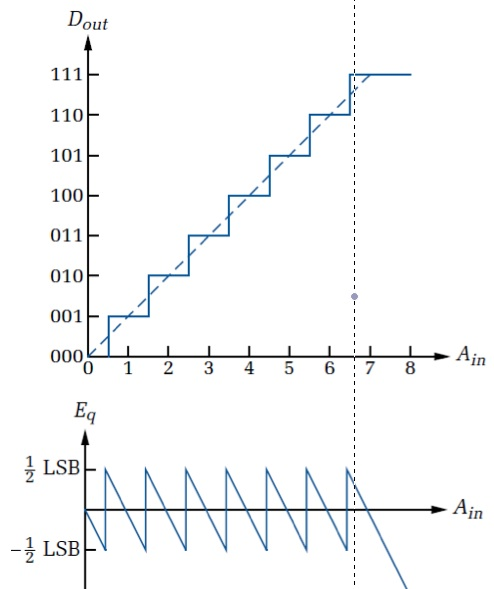
\includegraphics[height=5.9cm]{./pictures/idealerADC.jpg}}
	& \parbox[c]{0.31\textwidth}{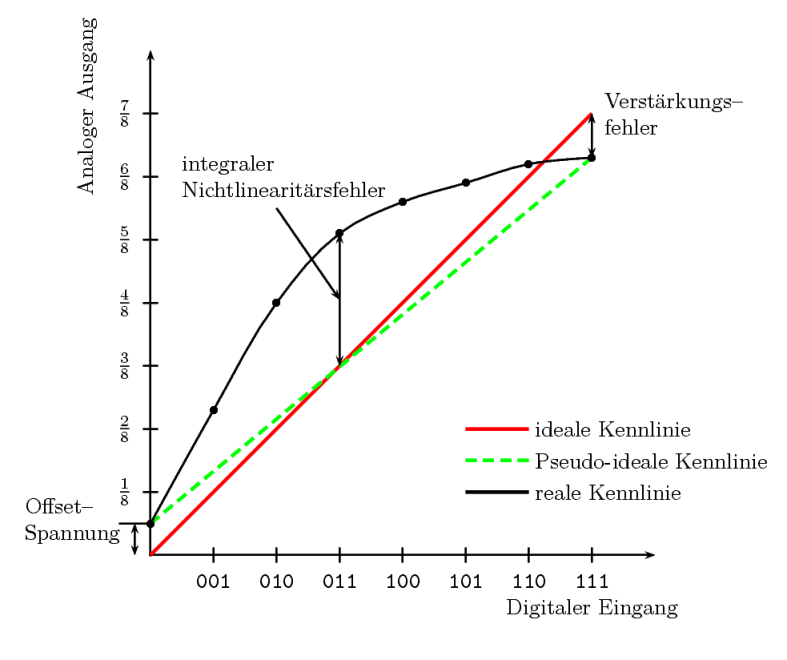
\includegraphics[width=0.31\textwidth]{./pictures/idealerDAC.png}}
	\\ \hline
	\textbf{Quantisierungsintervall}
	& $q = \frac{A_{max}}{2^N} = \frac{V_{refp}-V_{refn}}{2^N}$
	& $q = \frac{A_{Ref}}{2^N} = 1LSB $
	\\ \hline
	\textbf{Quantisierungsfehler}
	& $ -\frac{q}{2}\leq E_{q}<+\frac{q}{2} $
	&
	\\ \hline 
	\textbf{Ausgangsgrösse}
	&
	& $A_{out} = D_{in}*q = D_{in}*(\frac{A_{Ref}}{2^N})$
	\\ \hline
\end{tabular}


\subsection{Statische Fehler \hartl{434}}
\subsubsection{Offset-Fehler \hartl{434}}
Bei unipolaren A/D- bzw. D/A-Umsetzern sollte die digitale Null der
analogen Null entsprechen. In der Realität wird jedoch meistens eine Abweichung
aufgrund einer Verschiebung der Kennlinie auftreten. Diese wird als
Offset-Fehler bzw. Nullpunktfehler bezeichnet.
\begin{figure}[!ht]
\begin{center}
  \subfloat[ADC]{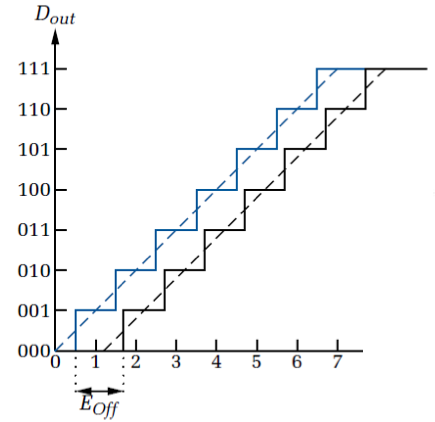
\includegraphics[width=6cm]{./pictures/EoffADC.png}}
  \subfloat[DAC]{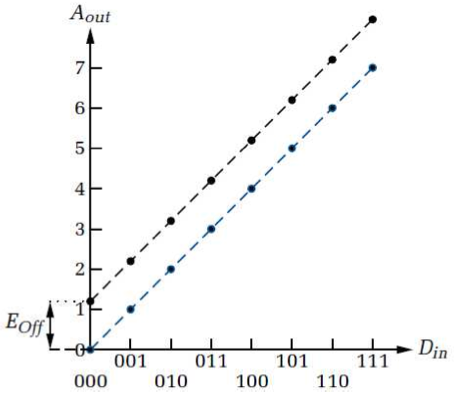
\includegraphics[width=6cm, height = 5cm]{./pictures/EoffDAC.png}}
\end{center}
\end{figure}

\subsubsection{Verstärkungsfehler\hartl{436}}
Eine Abweichung in der Steigung der
Kennlinie,gleichbedeutend mit der Verstärkung, verursacht beim realen Umsetzer eine Abweichung zur idealnen
Kennlinie. Diese Abweichung wächst mit jedem Quantisierungsschitt und führt beim
positiven Ende zum maximalen Fehler.
\begin{figure}[!ht]
\begin{center}
  \subfloat[ADC]{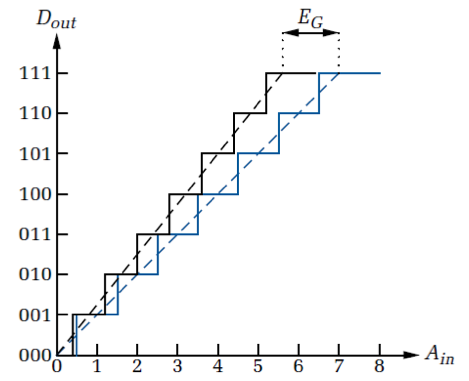
\includegraphics[width=6cm]{./pictures/verstaerkungsfehlerADC.png}}
  \subfloat[DAC]{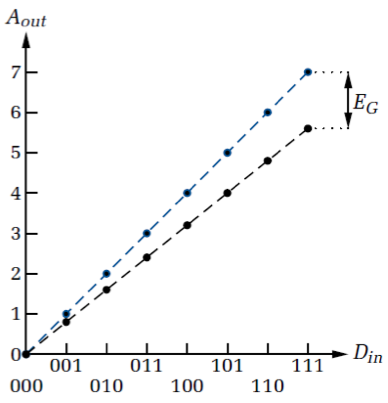
\includegraphics[width=6cm]{./pictures/verstaerkungsfehlerDAC.png}}
\end{center}
\end{figure}

\subsubsection{Differentielle Nichtlinearität DNL\hartl{437}}
Bei Offset- und Verstärkungsfehler wird von einer Verschiebung bzw.
konstanten Veränderung der Stufengrösse ausgegangen.Sobald aber die einzelnen
Stufen nicht mehr gleich gross sind, wird die Umsetzerkennlinie nicht linear.
Die differentielle Nichtlinearität beschreibt nun die Abweichung der einzelnen
Stufengrössen von der idealen.
\begin{figure}[!ht]
\begin{center}
  \subfloat[ADC]{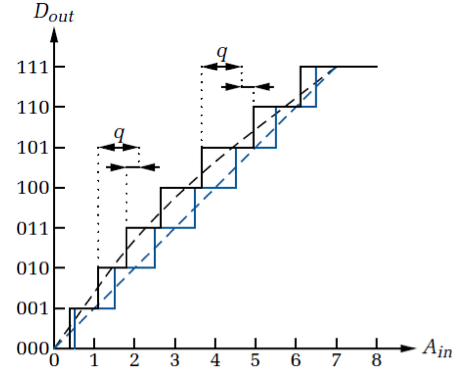
\includegraphics[width=6cm]{./pictures/DNL_ADC.png}}
  \subfloat[DAC]{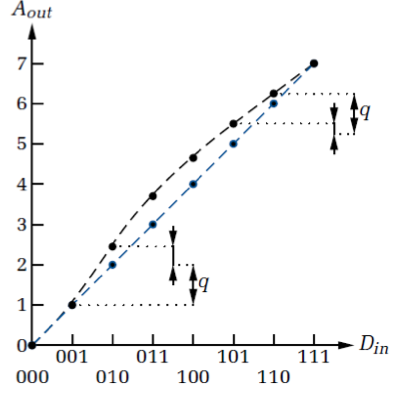
\includegraphics[width=6cm]{./pictures/DNL_DAC.png}}
\end{center}
\end{figure}

\subsubsection{Integrale Nichtlinearität INL \hartl{439}}
Bei der integralen Nichtlinearität wird die Abweichung der realen
Kennlinie zur idealen betrachtet. Damit wird der tatsächliche Fehler einer
Umsetzung beshrieben. Deshalb ist die integrale Nichtlinearität die wesentliche
Kengrösse zur Beschreibung der Linearität von A/D- bzw. D/A- Umsetzern. Wenn
von der Linearität eines Umsetzers gesprochen wird, ist (fast) immer die
integrale Nichtlinearität gemeint.
\begin{figure}[!ht]
\begin{center}
  \subfloat[ADC]{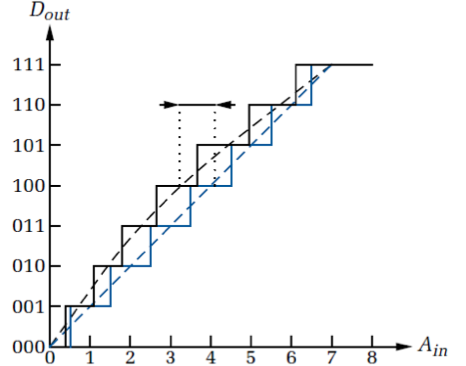
\includegraphics[width=6cm]{./pictures/INL_ADC.png}}
  \subfloat[DAC]{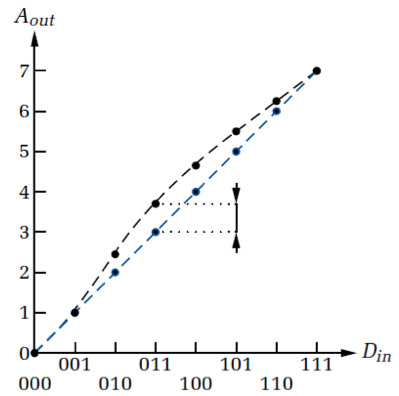
\includegraphics[width=6cm]{./pictures/INL_DAC.png}}
\end{center}
\end{figure}


\subsection{Eigenschaften und Fehler bei dynamischen Signalen\hartl{442}}
\subsubsection{Aperturfehler\hartl{442}} 
Bei einer periodischen Abtastung eines Signals ist immer ein gewisse zeitliche
Unsicherheit im Abtastzeitpunkt (Aperturunsicherheit) gegeben. Ist der Aperturfehler grösser als der maximal
auftretende Quantisierungsfehler ($\frac{1}{2}LSB$) so verschlechtert sich die Auflösung des Umsetzers. 


\begin{longtable}[c]{ l  l l l }
\begin{minipage}{4cm}

  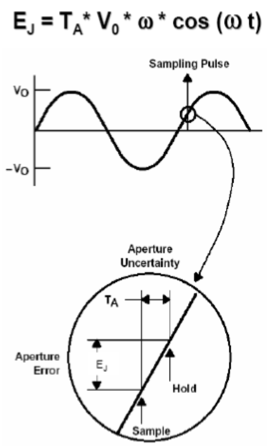
\includegraphics[scale=0.45]{pictures/aperturfehlercos}

\end{minipage}
&
\begin{minipage}{3cm}

  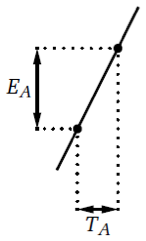
\includegraphics[scale=0.5]{pictures/aperturfehler}
\end{minipage}
&
\begin{minipage}{5cm}
\begin{gather}
x(t)=S\sin(2\pi ft)\\
\dot{x}(t)=2\pi fS\cos(2\pi t)\\
max\mid\dot{x}(t)\mid= 2\pi fS \\
E_{A}=2\pi fST_{A}\\
2S=A_{Ref}\\
E_{A}<E_{q}\\
E_{q}=\frac{q}{2}=\frac{A_{Ref}}{2*2^N}\\
E_{A}<\frac{A_{Ref}}{2*2^N}\\
2\pi fST_{A} <\frac{2S}{2*2^N}\\
T_{A}\frac{1}{\pi f2^{N+1}}
\end{gather}



\end{minipage}

&
\begin{minipage}{5cm}
\begin{tabular}{ll}
$E_{A}$: &Aperturfehler\\
$E_{q}$:&Quantisierungsfehler\\
$T_{A}$:&Zeitfehler\\
$A_{Ref}$:&analoge Referenz\\
N:& N bit Auflösung\\
S: &Amplitude\\
f: &Frequenz\\
t: &Zeit\\
x(t):&Signal
\end{tabular}


\end{minipage}
\\
\end{longtable}


\subsubsection{Aliasing}\hartl{444}
Aliasing entsteht bei Unterabtastung, d.h wenn das Abtasttheorem verletzt wird.
Es entstehen falsche, nur scheinbar vorhandene Komponenten im zeitdiskreten
Signal.\\
\\

\begin{tabular}{lll}
\small\textbf{Abtasttheorem}
&
\begin{minipage}{4cm}
\begin{equation}
f_{S}>2f_{max}
\end{equation}
\end{minipage}
&$f_{s}$: Abtastfrequenz\\
&&$f_{max}$:max. Frequenz des Signals
\end{tabular}

\subsection{Lineares Modell der Quantisierung}\hartl{448}
\subsubsection{Signal-Rausch-Verhältnis}\hartl{450}\\
\begin{tabular}{ll}

\begin{minipage}{10cm}
\begin{gather}
P_{Sig}=S^2_{Eff} =
\frac{S^2}{2}=\frac{(\frac{A_{Ref}}{2})^2}{2}=\frac{A^2_{Ref}}{8}\\
P^2_{N}=\frac{q^2}{12}=\frac{(\frac{A_{Ref}}{2^N})}{12}=\frac{A^2_{Ref}}{12*2^{2N}}\\
SNR=\frac{P^2_{S}}{P^2_{N}}=\frac{\frac{A^2_{Ref}}{8}}{\frac{A^2_{Ref}}{12*2^{2N}}}=\frac{12*2^{2N}}{8}=3*2^{2N-1}\\
SNR_{dB}=10\log(3*2^{2N-1})=6.02N+1.76dB\\
ENOB=\frac{SNR_{dB}-1.76}{6.02}
\end{gather}
\end{minipage}
&
\begin{minipage}{8cm}
\begin{tabular}{ll}
$P_{Sig}$:&Signalleistung\\
SNR:&Signal-Rausch-Verhältnis\\
$SNR_{dB}$:&Signal-Rausch-Verhältnis in dB\\
ENOB:&Effective Number of Bits\\
\end{tabular}
\end{minipage}
\end{tabular}
\newpage
\section{DA Wandler\hartl{455}}
  Es gibt 3 Verfahren: Parallelverfahren, Wägeverfahren und Zählverfahren.

\subsection{Parallelverfahren}

\renewcommand{\arraystretch}{1}
\begin{tabular}{|>{\bfseries}p{3cm}|c|p{6.6cm}|}
	\hline
	Strom-DAC \hartl{456} 
	& 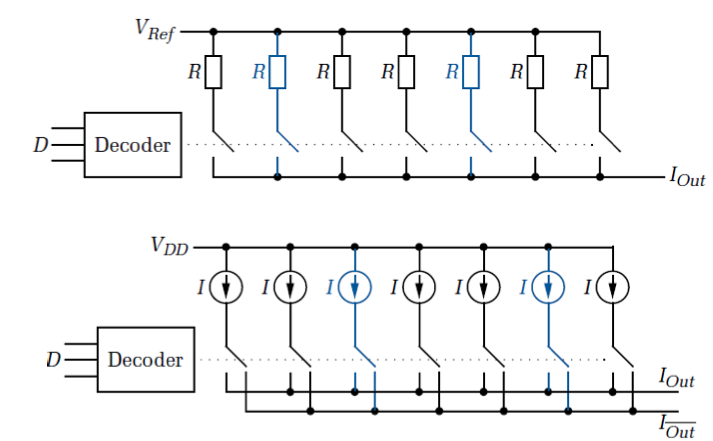
\includegraphics[width=7cm, valign=t]{pictures/Strom-DAC}
	& {\begin{align*}
      K &=2^N-1\\
      I &=\frac{V_{Ref}}{R} \qquad \text{(von einer Quelle)}
	  \end{align*}}
	  \begin{tabular}{lp{5cm}}
	  	K: & Anzahl Stromquellen \\
      D: & Eingangswert (Anzahl Schalter die aktiv sind.) \\
      \multicolumn{2}{l}{Schaltereigenschaften:}\\
      On: & kein Spannungsabfall  \\
      Off: & kein Strom
    \end{tabular} 
	\\ \hline
	String DAC (Voltage Scaling) \hartl{459}
	& 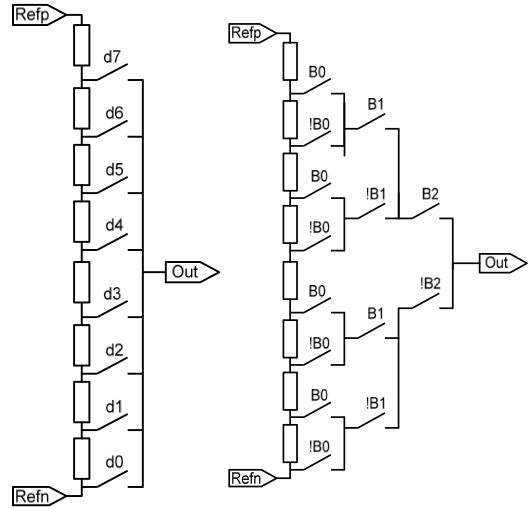
\includegraphics[width=5.5cm, valign=t]{pictures/string_DAC}
	& 
		\begin{description}
  		\item[Vorteile: ] garantierte Stetigkeit
  		\item[Nachteile:] benötigt $2^n$ Widerstände und $2^n$ Schalter, n-to-$2^n$ Decoder(linke Variante),
        er darf nicht belastet werden und hat ein grosser Schaltungsaufwand.
	  \end{description} 
    
	  {\begin{align*}
	  	V_{Out_{ideal}}(D) = \frac{D}{2^n}(V_{Refp}-V_{Refn})+V_{Refn}\\
	  	V_{Out_{real}}(D) = V_{Refn}+\left(V_{Refp}-V_{Refn}\right)\cdot\\
	  		\cdot\frac{D \cdot R_{Load}}{2^n \cdot R \cdot D-R \cdot D^2 + 2^n (R_{Load} + R_{Switch}) }\\
	  	DAC_{error}(D)=\frac{V_{Out_{real}}(D)-V_{Out_{ideal}}(D)}{V_{Out_{ideal}}(D)}\\
	  \end{align*}}
	  
	\\ \hline
	Segmented String DAC \hartl{459}
	& 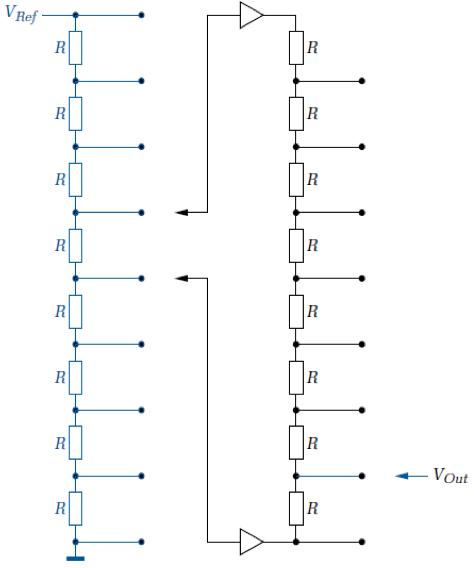
\includegraphics[width=5cm, height = 5cm, valign=t]{pictures/segmented_string_DAC}
	& \begin{description}
  		\item[Vorteile: ] viel weniger Elemente
  		\item[Nachteile:] benötigt Buffer (offset-frei)
	  \end{description}
	\\ \hline
\end{tabular}
\renewcommand{\arraystretch}{\arraystretchOriginal}

%\newpage

\subsection{Wägeverfahren\hartl{461}} 
\begin{longtable}{|p{3cm}|c|p{8.6cm}|}
	\hline
	\textbf{Spannungs"-summierung \hartl{461}}
	& 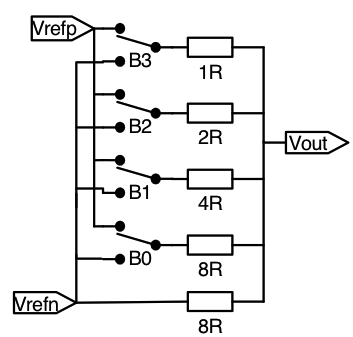
\includegraphics[width=5cm, valign=t]{./pictures/spannungssummierung.png}
	& {\begin{align*}
		V_{Out} &= \frac{B0\cdot 2^0 + B1 \cdot 2^1+ \ldots + B(n-1)\cdot 2^{n-1}}{2n} \\
    & \cdot (V_{Refp}-V_{Refn}) + V_{Refn}
	  \end{align*}}
    
	  \begin{description}
  		\item[Vorteile:] n Widerstände, n Schalter
  		\item[Nachteile:] nicht garantiert stetig, grosse Wertebereiche für Widerstände, rechnen mit Leitwerten ($G_0 = \frac{1}{8R}$)
	  \end{description}
	\\ \hline
	\textbf{Wägeverfahren mit Ausgangstreiber} \newline
  (Summation gewichteter Ströme)
	& 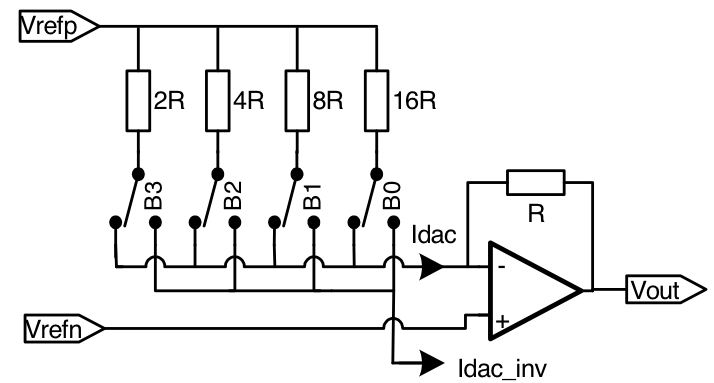
\includegraphics[width=6cm, valign=t]{./pictures/praktisch.png}
	& \[ Idac_{max}=\frac{V_{Refp}-V_{Refn}}{R} \cdot \frac{2^n-1}{2^n} \] \newline
    Vout und Idac\_inv sind differentiel zu einander, dadurch fliesst immer der gleiche Strom
    und der Offsetfehler bleibt konstant.
	\\ \hline
	\textbf{R-2R-Netzwerk \hartl{462}}
	& 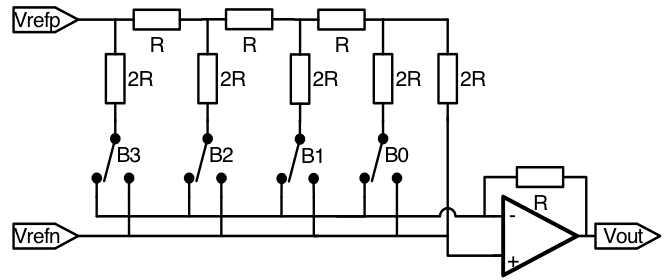
\includegraphics[width=6cm, valign=t]{./pictures/r2rnetzwerk.png}
	& {
	\begin{align*}
		V_{out,max} &= V_{Refn} \\
		V_{out,min} &= V_{Refn} - R \cdot I_{max}\\
		I_{max}		&= (V_{Refp} - V_{Refn}) (\frac{1}{2R} + \frac{1}{2}\frac{1}{2R} + \frac{1}{4} \frac{1}{2R} + \ldots) \\
					&= (V_{Refp} - V_{Refn})\frac{1}{2R}(2-2^{1-n})
	\end{align*}}
  
  \begin{description}
    \item[Vorteil:] nur 2 unterschiedliche R
    \item[Nachteil:] es muss immer ein Strom fliessen
  \end{description}
  
	\\ \hline
	\textbf{Kapazitiver DAC (Charge Scaling)}
	& 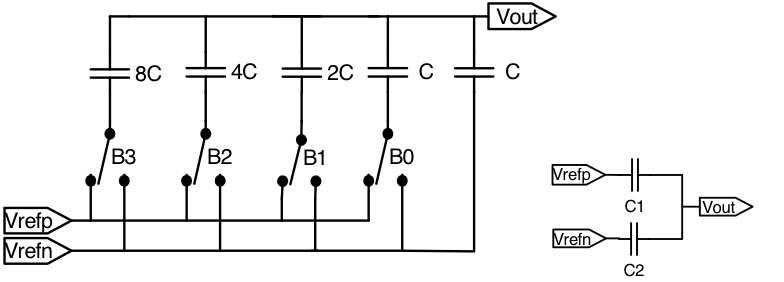
\includegraphics[width=6cm, valign=t]{./pictures/kapazitiverDAC.png}
	& {\begin{align*}
		C1	&= B3 \cdot 8C+B2 \cdot 4C+ B1 \cdot 2C+B0 \cdot C \\
		C2	&= !B3 \cdot 8C+!B2 \cdot 4C+ !B1 \cdot 2C+!B0 \cdot C+C \\
		V_{Out}& =\frac{C1}{C1+C2}\cdot (V_{Refp}-V_{Refn}) + V_{Refn}\\
		\text{mit } & C1+C2=2^n\cdot C
	  \end{align*}}
	\\ \hline
    \textbf{Kapazitiver DAC mit Ausgangstreiber}
    & 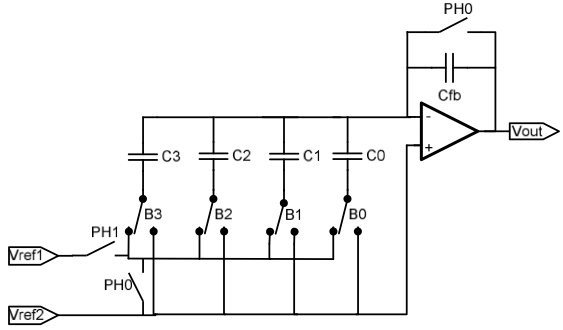
\includegraphics[width=6cm, valign=t]{./pictures/kapazitiverDACmitAmp.png}
    & {Wenn z.B. B3 auf $V_{Ref1}$ geschaltet wird:\newline
      \begin{align*}
          Q_{C3} = C_3 \cdot \Delta U &= C_3 \cdot (V_{Ref1}-V_{Ref2})\\
          \Delta Q_3 = \Delta Q_{fb} &= C_3 \cdot \Delta V_{Ref}\\
          \Rightarrow \Delta V_{Out} &= \frac{\Delta Q_{fb}}{C_{fb}} = \Delta V_{Ref} \cdot \frac{C_3}{C_{fb}}
      \end{align*}}
    \\ \hline
\end{longtable}

%\newpage

\subsection{Zählverfahren(PWM)\hartl{466}}
\begin{longtable}{|>{\bfseries}p{4cm}|l|p{8cm}|}
	\hline 
	Grundprinzip \hartl{466}
	& 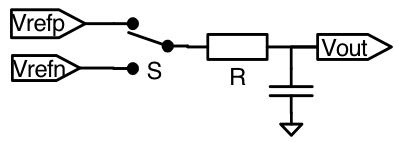
\includegraphics[width=6cm, valign=t]{./pictures/pwm_DAC.png}
	& $ V_{Out}=\frac{D}{2^n} \cdot (V_{Refp}-V_{Refn})+V_{Refn} $ \newline
	\begin{tabular}{lp{5cm}}
    \textbf{Vorteile:} 
      &-einfache Schaltung \\
      &-ermöglicht hohe Auflösung \\
      &-Funktioniert ohne analoge Schaltungen on Chip \\
    
    \textbf{Nachteile:}
      &-sehr langsam \\
      &-benötigt grosse Zeitkonstanten 
  \end{tabular}
	\\ \hline
	PWM-Ansteuerung \hartl{466}
	& \parbox[c][2cm]{6cm}{\begin{tikzpicture}[thick, transform shape, scale=0.55]
	\draw node at (0.5,0) [anchor=east] {$N$};
	\draw [->] (0.5,0) -- (1,0);
	\draw (1,0.5) rectangle (4,-0.5);
	\draw node at (2.5,0) {mod N Counter};
	
	\draw [->] (2.5,-0.5) -- (2.5,-1);
	
	\draw node at (0.5,-1.5) [anchor=east] {$N$};
	\draw [->] (0.5,-1.5) -- (1,-1.5);
	\draw (1,-1) rectangle (4,-2);
	\draw node at (2.5,-1.5) {$<n?$};
	
	\draw (4,-1.5) -- (4.5,-1.5) node [anchor=south] {Out};
	
	%PWM Signal:
	\node at (6,-1) [anchor=east] {$V_{ref}$};
	\node at (6,-1.5) [anchor=east] {$0$};
	
	\foreach \x in {6.5,8,8.5,10}
	{
		\draw (\x,-1) -- (\x,-1.5);
		\draw [dotted] (\x,-1) -- (\x,0);
	}
	\foreach \x in {6,8,10}
		\draw (\x,-1.5) -- (\x+0.5,-1.5);
	\foreach \x in {6.5,8.5}
		\draw (\x,-1) -- (\x+1.5,-1);
	
	\foreach \x in {6.5,8.5}
	{
		\draw [<->] (\x,0) -- (\x+2,0);
		\node at (\x+1,0) [anchor=south] {NT};
	}
	\foreach \x in {6.5,8.5}
	{
		\draw [<->] (\x,-0.5) -- (\x+1.5,-0.5);
		\node at (\x+0.75,-0.5) [anchor=south] {nT};
	}

\end{tikzpicture}}
	& $\bar{V_{Out}}=\frac{n}{N}V_{Ref}$
	  \begin{tabular}{ll}
		N:&Takte\\
		n:&digitale Eingangsgrösse
	  \end{tabular}
	\\ \hline
\end{longtable}

\newpage

\subsection{Weitere DAC}
\begin{longtable}{|>{\bfseries}p{4cm}|c|p{8cm}|}
	\hline
	Kaskadierte DAC
	& 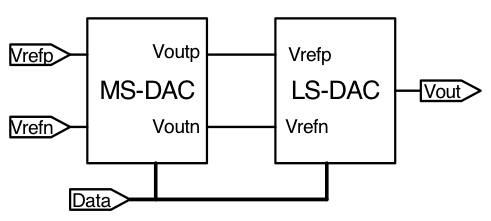
\includegraphics[width=6cm, valign=t]{./pictures/kaskadiertDAC.png}
	& \begin{itemize}
  		\item MS-DAC hat 2 Ausgangsspannungen (Über und unter dem gewünschten
  			$V_{Out}$)
  		\item LS-DAC hat kleine Eingangspannungsdifferenz $\to$ höhere Auflösung der
  			Spannung
	  \end{itemize}
	\\ \hline
	Zyklisch, algorithmischer DAC \hartl{466}
	& 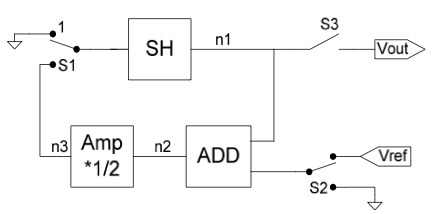
\includegraphics[width=6cm, valign=t]{./pictures/zyklischDAC.png}
	& \textbf{Ablauf der Wandlung}
	  \begin{enumerate}
  		\item Die Spannung im S/H löschen (Schalter S1), S3 offen)
  		\item S1 auf den Verstärker-Ausgang schalten
  		\item Laufvariale k wird auf 0 gesetzt
  		\item S2 setzen: VREF oder GND ( abh. $D_{K}$).
  		\item Der Addierer und Verstärker generieren Ausgangssignal
  		\item Im S/H wird die Feedback-Spannung gespeichert (S1)
  		\item X wird um 1 erhöht
  		\item Gehe zu Schritt 4, wenn $X\leq n$
	  \end{enumerate}
	\\ \hline
	Pipelined DAC 
	& 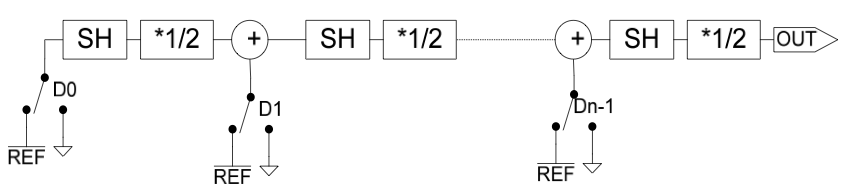
\includegraphics[width=6cm, valign=t]{pictures/piplinedDAC}
	& $V_{Out} = (D_0 \cdot 2^{-n} + D_1 \cdot 2^{1-n} + ... + D_{n-1} \cdot 2^{-1})\cdot V_{Ref}$\newline\newline
      Die Latenz beträgt n Zyklen, die Update-Frequenz ist aber n-mal grösser, da die Blöcke n-fach vorliegen.\newline
      LSB ($\mathrm{D_0}$): $\mathrm{V_{Ref}}$ wird n-mal halbiert
	\\ \hline
	Strom-DAC
	& 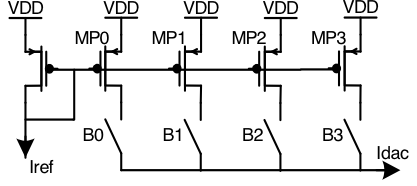
\includegraphics[width=6cm, valign=t]{pictures/stromDAC}
	& \begin{itemize}
  		\item Stromspiegel
  		\item MP0 ist gleich breit wie Stromquellen-MOS $\to \mathrm{I(MP0)=I_{Ref}} \qquad$ MP0: Einheitstransistor
  		\item MP1 ist doppelt so breit wie MP0 $\to \mathrm{I(MP1)}=2*\mathrm{I_{Ref}} \qquad$ MP1: 2 Einheitstransistoren
  		\item MP2 ist doppelt so breit wie MP1 $\to \mathrm{I(MP2)}=4*\mathrm{I_{Ref}} \qquad$ MP2: 4 Einheitstransistoren
  		\item \ldots
	  \end{itemize}
	\\ \hline
\end{longtable}

\subsection{Spezielle Wandler}
\begin{longtable}{|>{\bfseries}p{4cm}|c|p{8cm}|}
  \hline
    Digitales Potentiometer \hartl{460}
    & 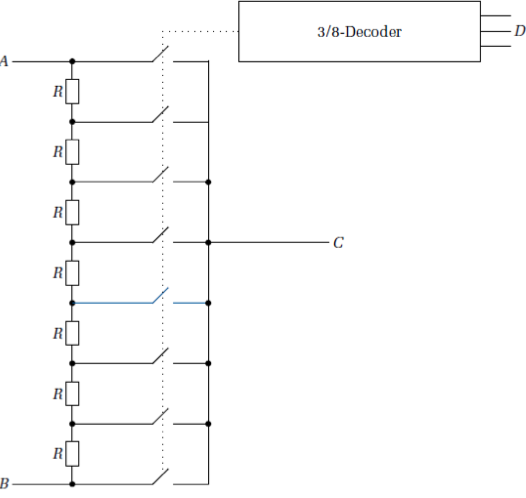
\includegraphics[width=5cm, valign=t]{pictures/digitales_potentiometer}
    & \begin{itemize}
        \item automatisierter Elektronik-Test möglich
        \item D (digitale Wert) wird im PROM gespeichert
        \item V(A), V(B) können variabel sein
      \end{itemize} \\
  \hline
    Multiplizierende Wandler
    & 
    & Wandler bei denen mit Widerständen aus der Referenzspannung Ströme abgeleitet werden.
    z.B R2R-Netzwerk \\
  \hline
    DAC mit Exponentieller Funktion
    &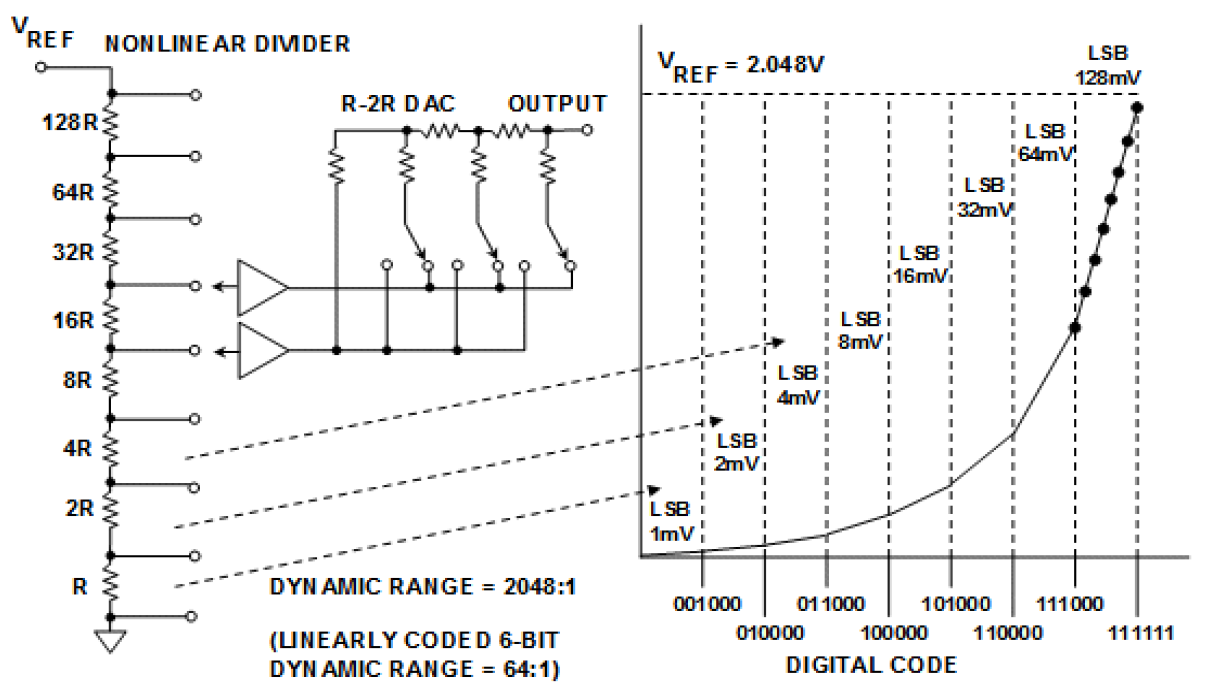
\includegraphics[width=6cm, valign=t]{pictures/DAC_exp.png}
    & \\
  \hline
\end{longtable}

\subsection{Ausgangsverstärker}
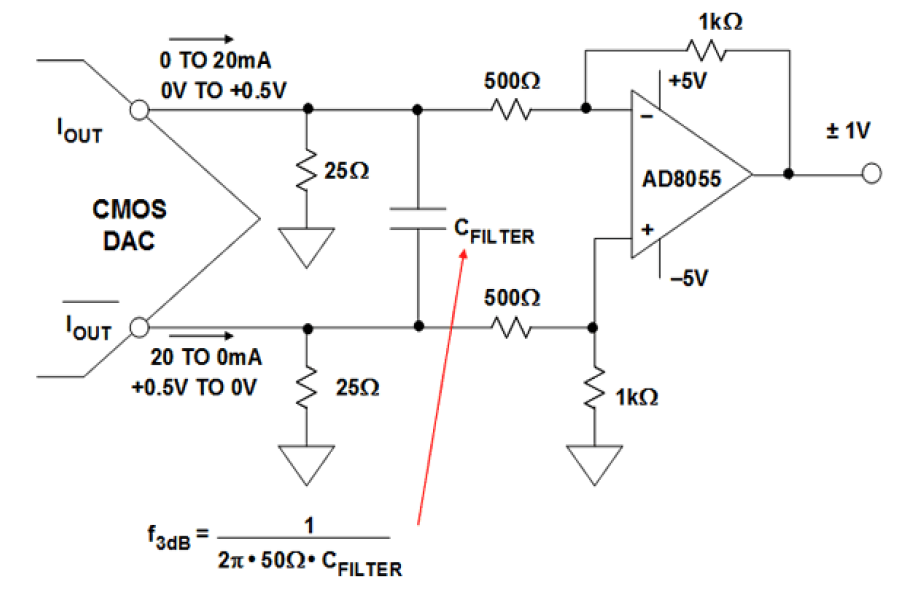
\includegraphics[width=6cm, valign=t]{pictures/Ausgangsverstaerker.png}

\section{AD Wandler \hartl{475}}

\subsection{Vergleich ADC}
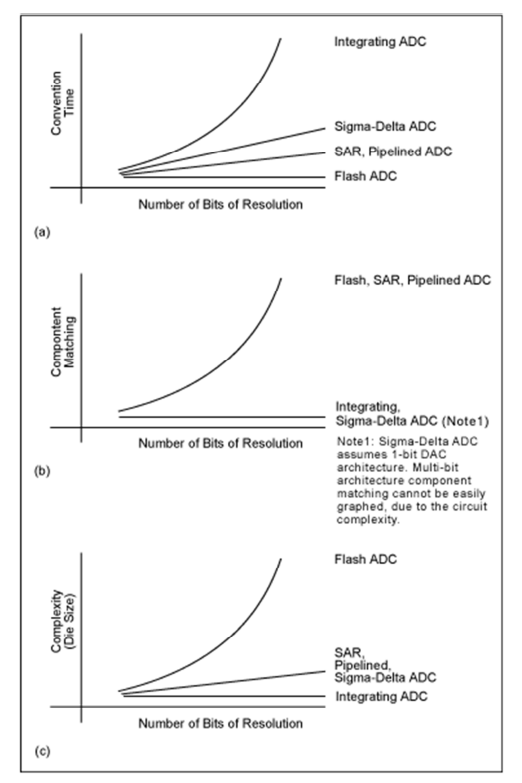
\includegraphics[width=9cm, valign=t]{pictures/vergleich_ADC.png}

\newpage

\subsection{Parallelverfahren und Kaskadenumsetzer}

\begin{longtable}{|>{\bfseries}p{4cm}|p{6cm}|p{8cm}|}
  \hline
    Parallelumsetzer (Flash-ADC) &
    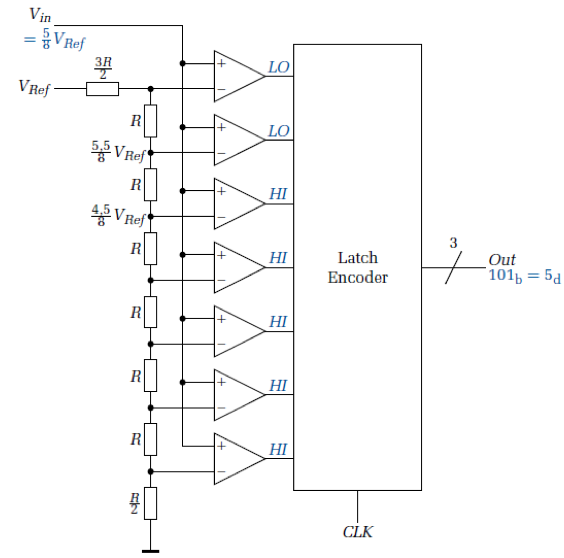
\includegraphics[width=6cm, valign=t]{pictures/parallelADC} &
    \begin{tabular}{ll}
      \textbf{Vorteile:} & sehr schnell \\
      & keine DAC Rückkopplung \\
      \textbf{Nachteile:} & geringe Auflösung \\
      & benötigt $2^n$ Widerstände \\
      & benötigt $2^n-1$ Komperatoren
    \end{tabular} \\
  \hline
    Kaskadenumsetzer (Pipeline ADC) &
    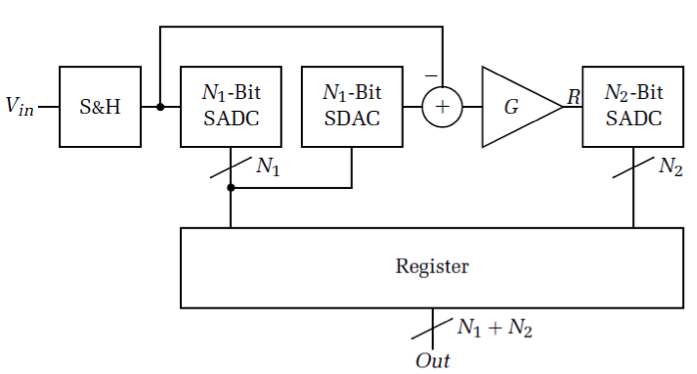
\includegraphics[width=6cm, valign=t]{pictures/kaskaden} \newline
    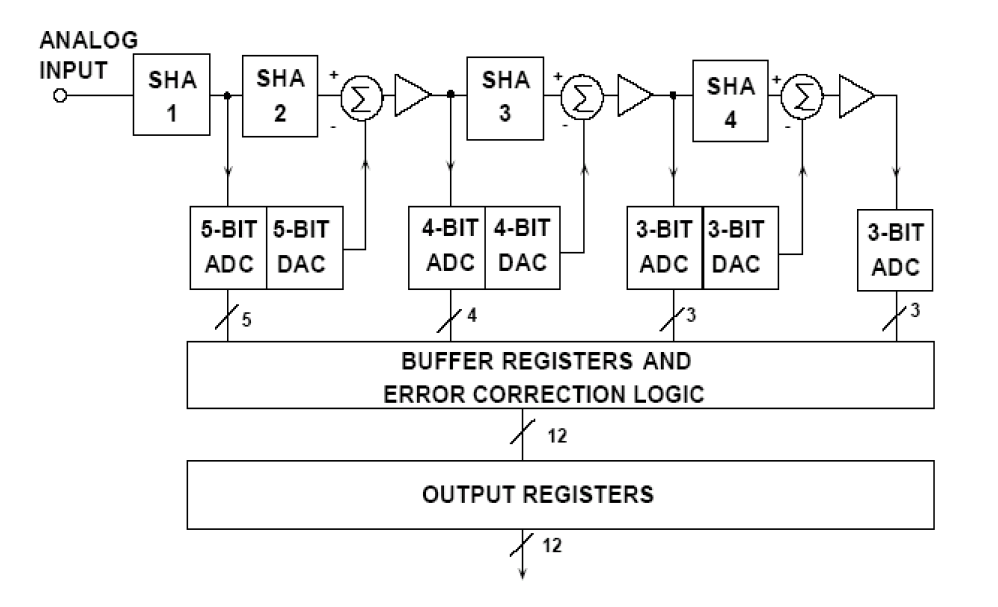
\includegraphics[width=6cm, valign=t]{pictures/kaskaden_fehlerkorrektur.png} \newline 
    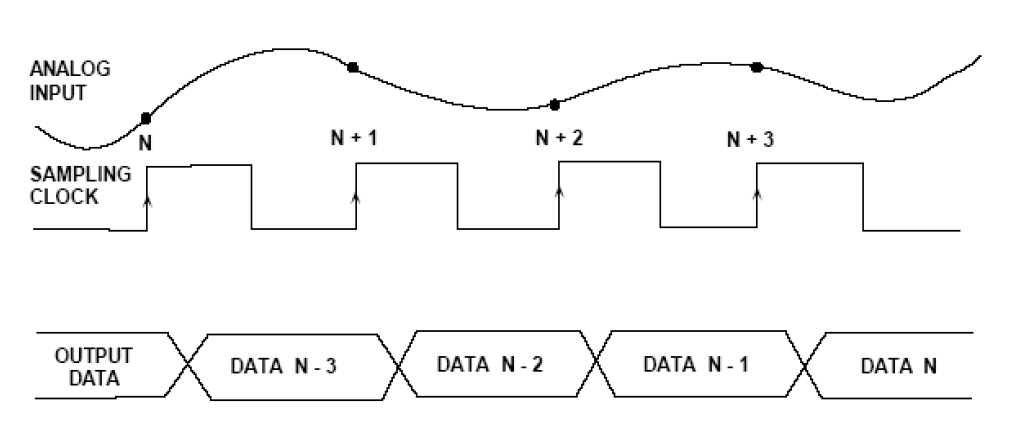
\includegraphics[width=6cm, valign=t]{pictures/latenz}&
    Eine 10-bit-Auflösung beim Parallelverfahren würde 1024 Komperatoren
    benötigen.$\Rightarrow$Komplexitätsreduktion \newline
    Mit erstem $N_{1}$-bit ADC wird der Grobbereich festgelegt (höherwertige
    Bits). Diese Zahl wird in eine analoge Spannung durch einen $N_{1}$-bit DAC zurück
    umgesetzt und diese Spannung von der Eingangsspannung subtrahiert. Diese
    Differenz wird von einem weiteren $N_{2}$-bit-ADC umgesetzt, um die
    niederwertigen Bits zu ergeben. Skaliert man die Differenzspannung mit dem
    Faktor 32, hat man den gleichen Spannungsbereich, kann also zwei identische
    ADC benutzen. \newline
    p = Anzahl Stufen \newline
    m = Bit pro Stufe \newline
    $p(2^m-1)$ Komperatoren \newline
    $n = p \cdot m$ \newline
    \newline
    \begin{tabular}{lp{6cm}}
      Bild 1: & Pipeline ADC ohne Fehlerkorrektur \\
      Bild 2: & Pipeline ADC mit Fehlerkorrektur \\
      Bild 3: & Verzögerung der Ausgangsdaten gegeüber den Sampels (Latenz)
    \end{tabular} \\
  \hline
\end{longtable}

\newpage

\subsection{Wägeverfahren (sukzessive Approximation/SAR) \hartl{485}}
\begin{longtable}{|>{\bfseries}p{4cm}|p{6cm}|p{8cm}|}
  \hline
    Prinip SAR &
    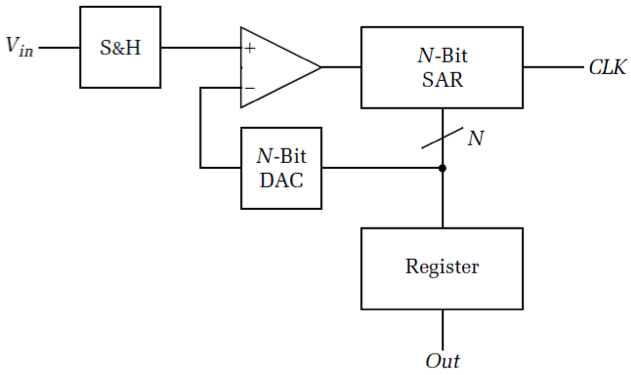
\includegraphics[width=6cm, valign=t]{pictures/waegeverfahren} &
    \begin{itemize}
      \item Abtastung der Eingangsspannung $V_{in}$mit einer
          S\&H-Schaltung( Vergleichsspannung liegt so während der gesamten
        Umsetzung an)
      \item Vergleich starte in der Mitte der Eingangsspannung $\frac{V_{Ref}}{2}$
    \end{itemize} \\
    
    &
    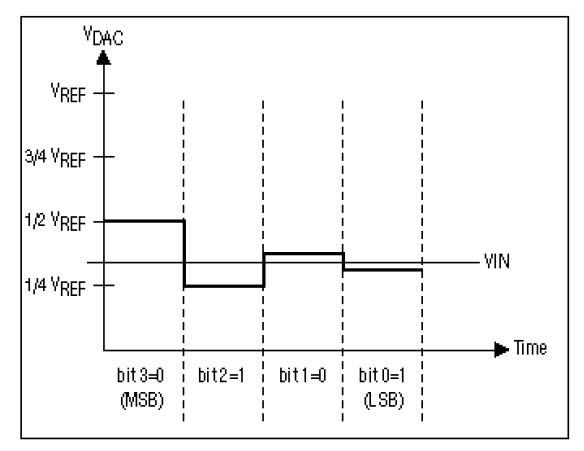
\includegraphics[width=6cm, valign=t]{pictures/prinzip_SAR.png} &
    \textbf{Ablauf der Wandlung:}
    \begin{enumerate}
      \item Im Sample-Hold wird ein analoger Wert gespeichert
      \item X(Laufvariable) wird auf n-1 gesetzt, DAC-Register wird auf 0 gsetzt
      \item Das Bit Bx vom DAC wird 1 gesetzt
      \item Komperator wird ausgewertet
            \begin{itemize}
              \item[1:] Bx = 1, DAC-Bit bleibt gesetzt
              \item[0:] Bx = 0, DAC-Bit wird gelöscht
            \end{itemize}
      \item X wird um 1 reduziert
      \item Gehe zu Schritt 3, wenn $X \geq 0$ 
    \end{enumerate} \\
  \hline
    Wägeverfahren mit SC-Prinzip &
    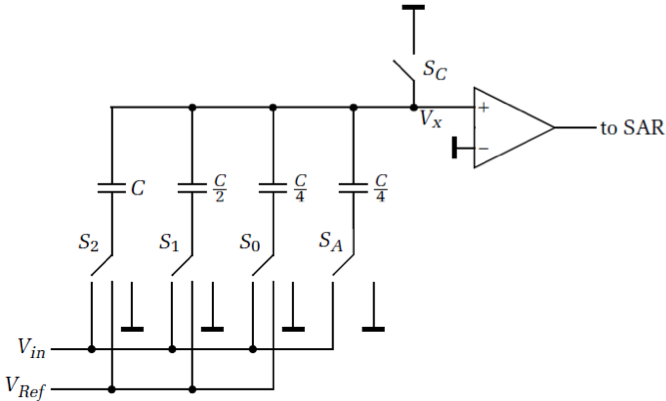
\includegraphics[width=6cm, valign=t]{pictures/waegeverfahrenSC} &
    \textbf{Ablauf der Wandlung:}
    \begin{enumerate}
      \item alle C mit $V_{in}$ laden
      \item $S_C$ öffnen
      \item $S_2, \ldots, S_A$ an $A_{GND}$
      \item Sukzessive $S_2, \ldots, S_0$ an $V_{Ref}$
    \end{enumerate}
    Wenn $S_2$ an $V_{Ref}$ ist gilt: $V_x = -V_{in}+\frac{V_{Ref}}{2}$ \\
  \hline
\end{longtable}


\subsection{Iterative ADC}
\begin{longtable}{|p{12cm}|p{6cm}|}
  \hline
    \begin{enumerate}
      \item Im S/H wird die Eingangsspannung geschpeichert (Schalter Sin)
      \item Schalter Sin wird danach auf den Multiplizierer-Ausgang geschaltet
      \item X(Laufvariable) wird auf n-1 gesetzt
      \item Der Komparator wird ausgewertet\newline
        Dout=1: Bx=1, Switch S=1 (d.h. im Subtrahierer wird Vrefh von Vc
        subtrahiert)\newline
        Dout=0: Bx=0, Switch S=0 (d.h. im Subtrahierer wird 0 von Vc
        subtrahiert)
      \item Der Subtrahierer generiert sein Ausgangssignal
      \item Der Multiplizierer generiert sein Ausgangssignal
      \item Im S/H wird die Feedback-Spannung gespeichert (Schalter Sin)
      \item X wird um 1 reduziert
      \item Gehe zu Schritt 4, wenn $X\geq0$
    \end{enumerate} &
    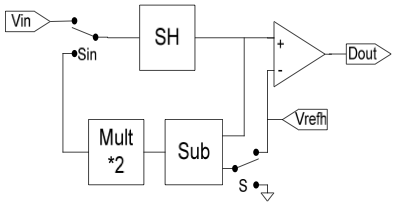
\includegraphics[width=6cm, valign=t]{pictures/iterativeADC}\newline
    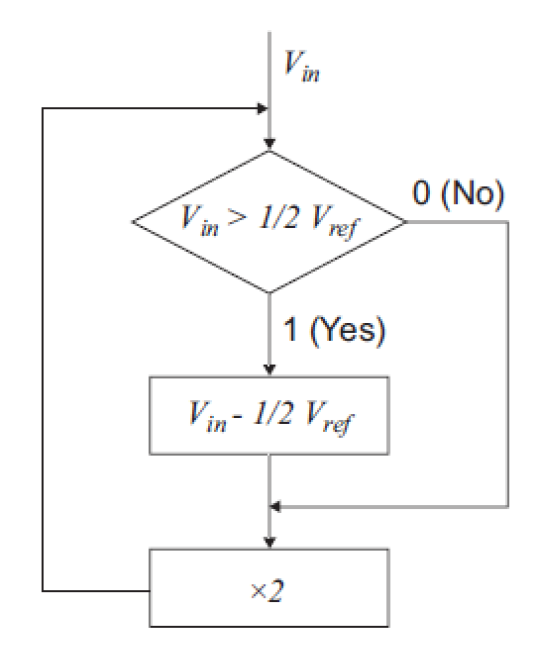
\includegraphics[width=6cm, valign=t]{pictures/iterativeADC_ablauf}\\
  \hline
\end{longtable}



\subsection{Zählverfahren \hartl{490}} 
Ist für kontinuierliche Auswertungen des Eingangssignal
\subsubsection{Single Slope}

\begin{tabular}{ccp{4cm}}
  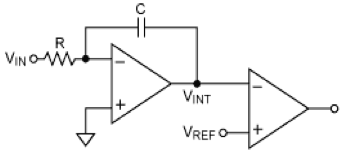
\includegraphics[width=6cm, valign=t]{pictures/singleSlope1} &
  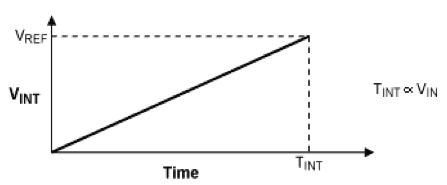
\includegraphics[width=6cm, valign=t]{pictures/singleSlope2} &
  {\begin{align*}
    V_{in}=\frac{V_{Ref} \cdot R \cdot C}{T_{int}}
  \end{align*}} \\
\end{tabular}

\subsubsection{Dual Slope \hartl{492}}
\begin{longtable}{cp{12cm}}
  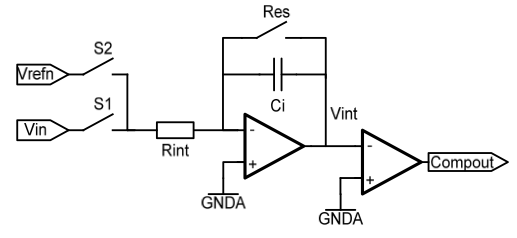
\includegraphics[width=6cm, valign=t]{pictures/dualSlope11} &
  $T_{int} = const$ \newline
  \[ V_{int} = V_{AGND} - \frac{1}{R_i \cdot C_i} \cdot T_{int} \cdot (V_{in} - V_{AGND})\] \\
 
  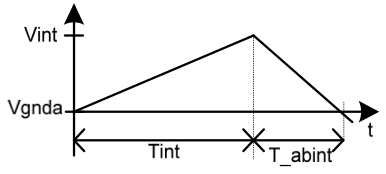
\includegraphics[width=6cm, valign=t]{pictures/dualSlope12} &
  \begin{tabular}{p{6cm}p{6cm}}
      \textbf{Integration:} &
      \textbf{Abintegration:} \\
  
      \[ V_{int_{max}} = - \dfrac{1}{R_i \cdot C_i} \cdot V_{in1} \cdot T_{int} \] &
      \[ V_{int}(t) = V_{int_{max}} - \dfrac{V_{Ref}}{R_i \cdot C_i}\cdot t \] 
  \end{tabular} \\
  
  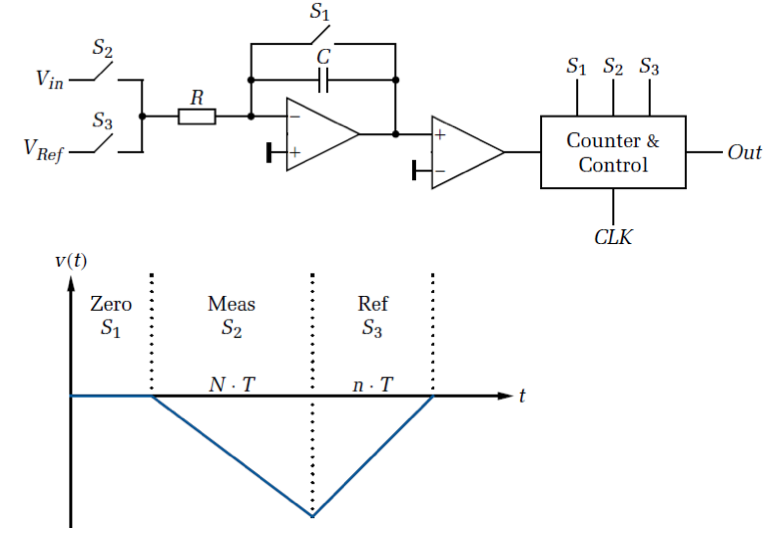
\includegraphics[width=6cm, valign=t]{pictures/dualSlope2} &
  \begin{tabular}{p{4cm}p{7cm}}
      \textbf{Abintegrationszeit:} &
      \textbf{Auflösung in Bits:} \\
  
      \[ t_{ab_{int}} = -\dfrac{V_{in1} \cdot T_{int}}{V_{Ref}} \] &
      \[ n = \dfrac{\log (\text{max Taktzyklen von Abintegration})}{\log(2)} \] 
  \end{tabular}
  \[ V_{in} = \frac{n}{N} \cdot V_{ref} \]
  
 Sinusschwingungen mit einer Periodendauer gleich der Integrationszeit, werden herausgefiltert!\\
 
  \begin{tabular}{ll}
    N:&Taktzyklen\\
    T:&Periodendauer\\
    n:&Zählerstand\\
    $V_{off}$:&Offsetspannung\\
  \end{tabular} &
  
  \begin{tabular}{ll}
    $T_{int}$:&Integrationszeit (ist vorgegeben)\\
    $T_{abint}$:& "`Messzeit"\\
    $V_{int}$:&Spannung am $V_{opOut}$ nach der Zeit $T_{int}$\\
    $V_{intmax}:$&maximal mögliche Spannung am $V_{opOut}$\\
  \end{tabular}
\end{longtable}

\begin{longtable}{p{4cm}p{6cm}p{8cm}}
  \textbf{Offsetkompensation:} &
  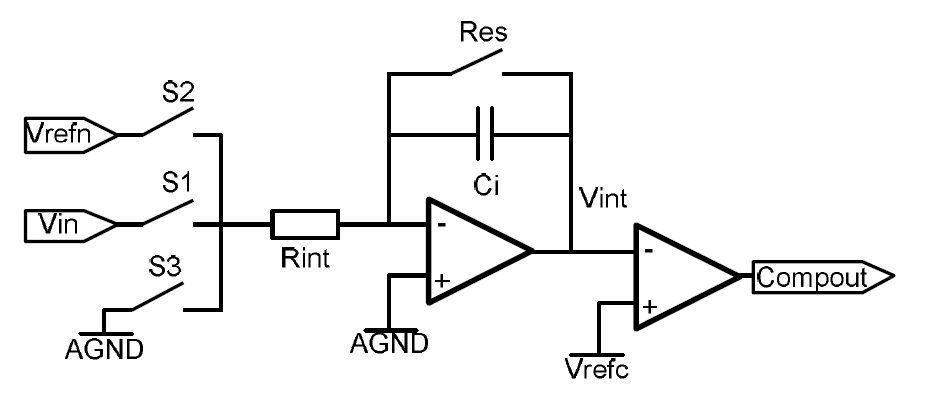
\includegraphics[width=6cm, valign=t]{pictures/offsetkompensation} &
  \textbf{Möglichkeiten zur Korrektur:}
  \begin{itemize}
    \item 2.Referenzspannung $V_{Refp}$ einfügen
    \item Die Komperator-Schwelle $V_{Refc}$ negativ gegeüber $AGND$ verschieben
    \item Dem OP einen Offset in einer Richtung vorgeben, damit er max 0 sein kann.
  \end{itemize}
\end{longtable}

\newpage

\subsubsection{Sigma-Delta Wandler \hartl{500}}
  \begin{longtable}{p{6cm}p{12cm}}
    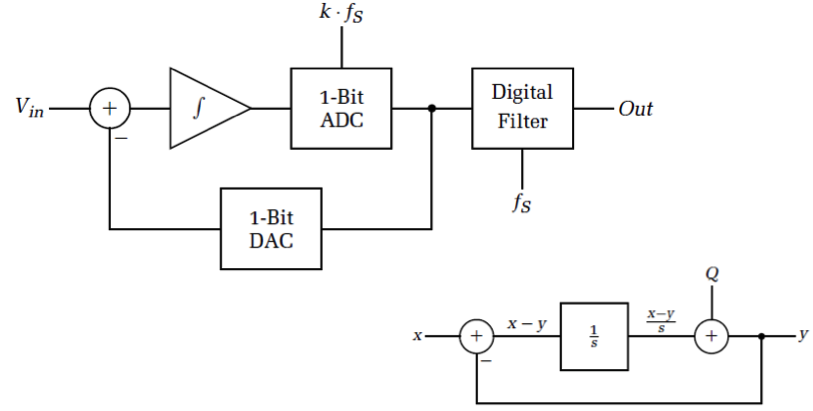
\includegraphics[width=6cm, valign=t]{pictures/deltaSigma1} \newline 
    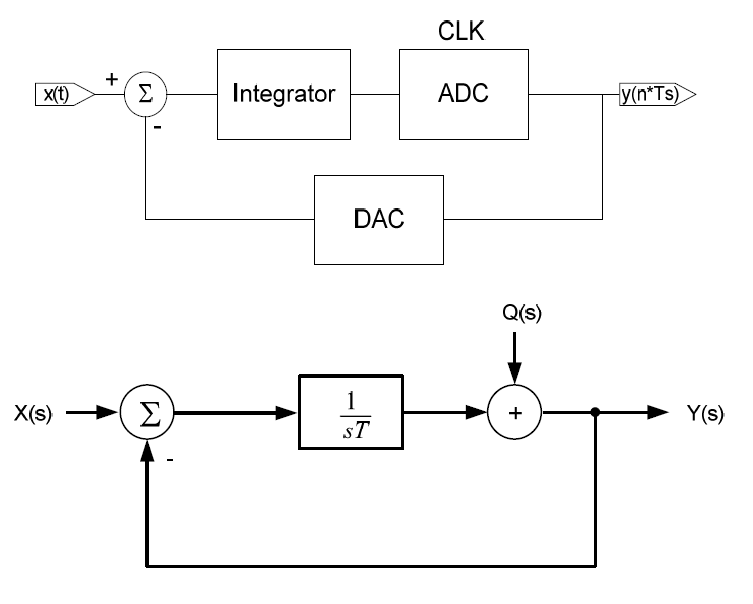
\includegraphics[width=6cm]{pictures/deltaSigma3} &
    \[Y=\frac{X-Y}{s}+Q\Rightarrow Y=X\frac{1}{1+s}+Q\frac{s}{1+s}\] \newline
    \begin{tabular}{p{3cm}p{9cm}}
      \textbf{Signal UTF:} &
      \textbf{Noise UTF:} \\
      
      \[ H_s(s) = \frac{1}{1+sT} \] &    
      \[ H_n(s) = \frac{sT}{1+sT} \] \\ \\
      
      SNR-Erhöhung: &
      $9dB$ oder 1.5Bit pro Verdoppelung des OSR (OverSamplingRatio) \\
      Hauptnachteil: &
      Pattern Noise (repetitive Sequenzen, die nicht von Signalen unterschieden werden können)
    \end{tabular}
    $Q(s)$ = Quantisierungsrauschen
    
  \end{longtable}

  %\begin{longtable}{cp{12cm}}
    %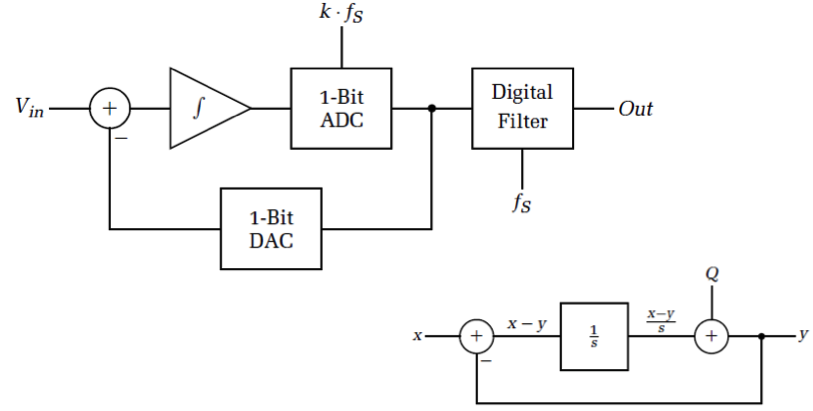
\includegraphics[width=6cm, valign=t]{pictures/deltaSigma1} &
    %\[Y=\frac{X-Y}{s}+Q\Rightarrow Y=X\frac{1}{1+s}+Q\frac{s}{1+s}\] \\
  %
    %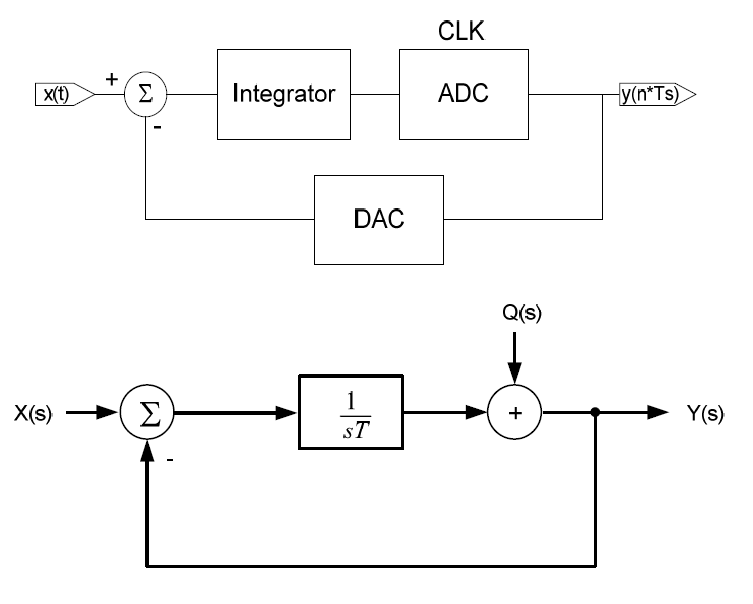
\includegraphics[width=6cm]{pictures/deltaSigma3} &
    %\begin{tabular}{p{3cm}p{9cm}}
      %\textbf{Signal UTF:} &
      %\textbf{Noise UTF:} \\
      %
      %\[ H_s(s) = \frac{1}{1+sT} \] &    
      %\[ H_n(s) = \frac{sT}{1+sT} \] \\ \\
      %
      %SNR-Erhöhung: &
      %$9dB$ oder 1.5Bit pro Verdoppelung des OSR (OverSamplingRatio) \\
      %Hauptnachteil: &
      %Pattern Noise (repetitive Sequenzen, die nicht von Signalen unterschieden werden können)
    %\end{tabular}
    %$Q(s)$ = Quantisierungsrauschen \newline
    %
  %\end{longtable}
	

%\subsubsection{Spannungs- Frequenz- Umsetzer \hartl{495}}
%\begin{multicols}{2}
	%\begin{center}
  		%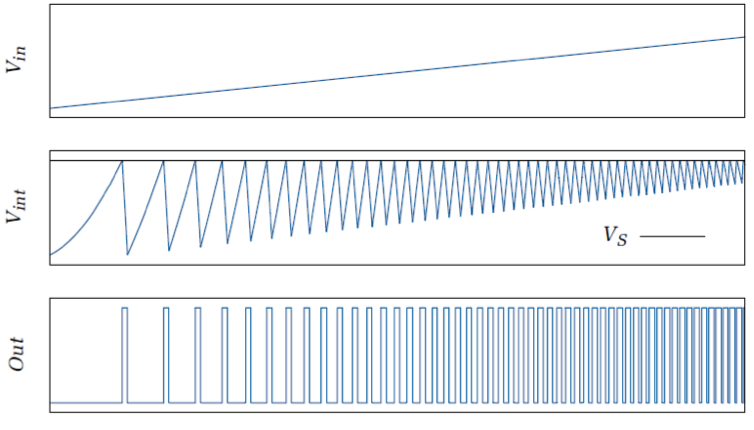
\includegraphics[width=7cm]{pictures/sfu_kurven}
  	%\end{center}
  %
  %
  %\includegraphics[width=6cm]{pictures/sfu_schaltung}
  %
   %\begin{align*}
      %V_{int}(t)=V_{in}+\frac{1}{RC}\int(V_{in}-V_{x})dt
   %\end{align*}
    %Vorteil: Immer am Eingangssignal\newline
    %Nachteil: Kein echter ADC  


%\subsubsection{Ladungs-Ausgleichs-Integrator \hartl{497}}
	%\includegraphics[width=6cm, valign=t]{pictures/lsg1} \\
	%\includegraphics[width=6cm, valign=t]{pictures/lsg2}
	%\begin{itemize}
	   %\item Gleichgewichtsbedingung\\
	    %\begin{equation*}
	      %V_{in}-\frac{n}{N}V_{Ref}=0\Rightarrow n=\frac{V_{in}}{V_{Ref}}N
	    %\end{equation*}
	  %\item Flipflop statt Monoflop
	%\end{itemize}
%\end{multicols}	

\begin{multicols}{2}
  \subsubsection{Sigma-Delta Wandler 2. Ordnung}
    \includegraphics[width=6cm, height =4cm]{pictures/deltaSigma2}
  
  \columnbreak
  
  \subsubsection{PWM vs. Sigma-Delta}
      \textbf{Digitalteil PWM}
      \begin{itemize}
        \item Zähler zählt bis $2^n$
        \item Komperator schaltet Ausgang
        \item '1' sind hintereinander
      \end{itemize}
      
      \textbf{Digitalteil Sigma-Delta DAC}
      \begin{itemize}
        \item Dig.wert wird "`integriert"'
        \item Übertrag schaltet Ausgang
        \item '1' werden verteilt
      \end{itemize}
\end{multicols}

\subsection{Dynamikbereich}
\subsubsection{Dithering}
  Ein Signal kann mittel Mittelwertbildung höher aufgelöst werden, wenn es mit Rauschen überlager ist.
  Die Auflösung wird gegen Bandbreite "`eingetauscht"' (Die Rauschleistung wird auf die Bandbreite aufgeteilt,
  dadurch ist nur noch ein kleiner Rauschanteil im Signalband).
  
\subsubsection{Oversampling}
  \begin{tabular}{lll}
    Over Sampling Ratio: &
    $OSR = \dfrac{f_s}{2+f_{max}}$ & \\
    
    Signal to Noise Ratio: &
    $SNR_{dB} = 1.76dB + n \cdot 6.02dB$ &
    (ohne Überabtastung)\\
    
    & $SNR_{dB} = 1.76dB + n \cdot 6.02dB + 10 \cdot \log (OSR)$ &
    (mit Überabtastung)
  \end{tabular}
  
  Durch Überabtastung wird das Quantisierungsrauschen über einen grösseren Frequenzbereich verteilt.
  Da die Rauschleistungsdichte ($=q^2/12$) konstant ist, wird durch eine grössere Bandbreite die
  Rauschleistungsdichte kleiner.
  
\subsubsection{Effektive Bit-Zahl (ENOB)}
  \begin{tabular}{lp{8cm}}
    Signal to Noise and Distortion: &
    \[SINAD = 10 \cdot \log \left(\dfrac{P_{signal}+P_{noise}+P_{distortion}}{P_{noise}+P_{distortion}}\right)\] \\
    Effective Number of Bits: &
    \[ENOB = \dfrac{SINAD-1.76}{6.02}\]
  \end{tabular}

  
  



\newpage
\newpage
\section{OpAmps AC}

Der Operationsverstärker ist in allgemeiner Näherung ein Tiefpass-Filter n-ter Ordnung mit linearer Verstärkung.

 \begin{tabular}{|p{0.15\linewidth}|p{0.28\linewidth}|p{0.445\linewidth}|}
 	\hline
 	Frequenzgang allgemein
 		& \large{$A(s) = \frac{A_{0}}{(1+\frac{s}{\omega_{p_1}})(1+\frac{s}{\omega_{p_2}})\dots}$}
 		& $A_{0}=$ Lineare Verstärkung \newline $\omega{p_i}=$ Polkreisfrequenzen \\
 	\hline
 \end{tabular}
 
\subsection{Open-Loop/Closed-Loop Verhalten}

\begin{tabular}{|p{0.45\linewidth}|p{0.45\linewidth}|}
	\hline
	\textbf{Open-Loop}
		& \textbf{Closed-Loop}\\
	\hline
	\multicolumn{2}{|c|}{\textbf{Blockschemas}}\\
	\hline
    \vspace{-7mm}
	\begin{center}
	 	\includegraphics[height=2cm, valign=t]{./pictures/opAmpOL.png}
	\end{center}
		& \vspace{-7mm}
          \begin{center}
			\includegraphics[height=2cm, valign=t]{./pictures/opAmpCL.png}
		  \end{center}\\
	\hline
	\multicolumn{2}{|c|}{\textbf{Frequenzgänge}}\\
	\hline
	\large{$A_{ol}(s)=\frac{A_{ol_0}}{(1+\frac{s}{\omega_{p_{ol_1}}})(1+\frac{s}{\omega_{p_{ol_2}}})\dots}$}
	& $\begin{aligned}
        A_{cl}(s) &= \frac{A_{cl_0}}{(1+\frac{s}{\omega_{p_{cl_1}}})(1+\frac{s}{\omega_{p_{cl_2}}})\dots} = \frac{T_{in}\cdot A_{ol_0}}{1+\beta(s)\cdot A_{ol_0}}\\
		\beta(s) &= \frac{U_{opn}}{U_{out}}\;\text{oder}\;\frac{U_{opp}}{U_{out}}\\
		T_{in}(s) &= \frac{U_{opn}}{U_{in}}\;\text{oder}\;\frac{U_{opp}}{U_{in}}\\
        U_{out} &= A_{cl}(s)\cdot U_{in} = \frac{T_{in}(s)\cdot A(s)}{1 + \underbrace{A(s)\cdot \beta(s)}_{T_s(s):Loop-Gain}} \cdot U_{in}
	   \end{aligned}$\\
	\hline
\end{tabular}
\\ \\
\begin{tabular}{m{0.45\linewidth}m{0.45\linewidth}}
	Durch das Schliessen des Loops wird die Bandbreite vergrössert, das gain-bandwidth-product(GBP) bleibt jedoch konstant. Die Verstärkung wird jedoch um $Tf_0(s)$ reduziert. Der Phasengang wird durch das Verschieben des ersten Poles auch verändert, wie folgende Grafik zeigt.
	& \begin{center}
        \includegraphics[width=6.7cm, valign=t]{./pictures/AolAcl.png}
    \end{center}
\end{tabular}
\vspace{-7mm}
\subsection{Stabilität des Systems}
\begin{tabular}{m{0.45\linewidth}m{0.45\linewidth}}
    Um die Stabilität des OpAmps zu betrachten, wird der Loop geöffnet. Damit das System stabil ist, darf das       
    Fehlersignal sich selbst nicht verstärken. Damit dies der Fall ist muss der Loop gain bei einer Phase von $-180^\circ$
    nicht $>1$ sein, da das Vergleichsglied die Phase noch um $180^\circ$ dreht. Ein Mass für die Stabilität ist die 
    Phasenmarge (Phase Margin) und die Verstärkungsmarge (Gain Margin). Optimal ist ein Phase Margin von $60^{\circ}$.
    
    Die UTF ist dann stabil, wenn sie nie $\infty$ wird d.h der Nenner darf nie 0 werden.
    & \begin{center}
        \includegraphics[width=6.7cm, valign=t]{./pictures/margins.png}
    \end{center}
\end{tabular}

% ----------------------------------------------------------------------------------------------------  
\subsection{OP als Regelkreis}  
\vspace{-1.5\topsep}
\begin{longtable}[t]{|p{5cm}|p{12.7cm}|}
    \hline  
    \multicolumn{2}{|l|}{\bf Nicht-invertierender OP}
    \\ \hdashline
    \includegraphics[width=5cm, valign=t]{pictures/opAmpNI.png}\newline\newline
    \includegraphics[width=5cm]{pictures/OPnichtInv.png}
    & {\vspace{-1.5\topsep}
        \begin{align*}
            A &= A_{ol}\\
            T_{in} &= 1\\
            \beta &= \frac{R_1}{R_1 + R_f}\\
            \frac{V_{out}}{V_{in}} &= \textcolor{red}{T = \frac{T_{in}}{\beta}\cdot \frac{1}{1+ \frac{1}{\beta 
            \cdot A_{ol}}} = \frac{T_{in}\cdot A_{ol}}{1 + A_{ol}\cdot \beta}} = 
            \frac{A_{ol}}{1 + A_{ol} \cdot \frac{R_1}{R_1 + R_f}} \approx \frac{R_1 + R_f}{R_1} =\frac{1}{\beta}
        \end{align*}
    }
    \\ \hline
% ---------------------------------------------------------------------------------------------------- 
    \multicolumn{2}{|l|}{\bf Invertierender OP}
    \\ \hdashline
    \includegraphics[width=5cm, valign=t]{pictures/opAmpInv.png}\newline\newline
    \includegraphics[width=5cm]{pictures/OPInv.png}
    & {\vspace{-1.5\topsep}
        \begin{align*}
            A &= A_{ol}\\
            T_{in} &= \frac{R_f}{R_1 + R_f} = 1 - \beta\\
            \beta &= \frac{R_1}{R_1 + R_f}\\
            \frac{V_{out}}{V_{in}} &= \textcolor{red}{T = -\frac{T_{in}}{\beta}\cdot 
            \frac{1}{1+ \frac{1}{\beta \cdot A_{ol}}}} =
            \frac{-T_{in} \cdot A_{ol}}{1+A_{ol} \cdot \beta}\approx -\frac{R_f}{R_1} = -\frac{1-\beta}{\beta}
        \end{align*}
    }
    \\ \hline
\end{longtable}
% ---------------------------------------------------------------------------------------------------- 
\vspace{-2.5\topsep}
\begin{longtable}[t]{|p{5cm}|p{12.7cm}|}
    \hline  
    \multicolumn{2}{|l|}{\bf Closed-Loop-Frequenzgang}
    \\ \hdashline
    \includegraphics[width=5cm, valign=t]{pictures/ClosedLoopFreqGang.png}
    & {\vspace{-1.5\topsep}
        \begin{align*}
            \intertext{Frequenzabhängige Verstärkung Opamp:}
            A_{ol}(s) &= \frac{A_0}{1 + s/\omega_p}\\
            \intertext{eingesetzt in folgende Formel:}
            V_{out} &= \frac{A_{ol}}{1 + \beta \cdot A_{ol}} \cdot V_{in}\\
            \intertext{ergibt:}
            A_{cl}(s) &= \frac{\frac{A_0}{1 + s/\omega_p}}{1 + \beta \frac{A_0}{1 + s/\omega_p}} = 
            \frac{A_0}{(1 + A_0 \beta) + s/\omega_p} = 
            \frac{\textcolor{red}{\frac{A_0}{1 + A_0 \beta}}}{1 + s \frac{1}
            {\textcolor{blue}{\omega_p(1 + A_0 \beta)}}} = 
            \frac{\textcolor{red}{A_{0_{cl}}}}{1 + s\frac{1}{\textcolor{blue}{\omega_{p_{cl}}}}}
        \end{align*}
        \newline
        Für $\mathrm{A_0 \cdot \beta \gg 1}$ gilt:\newline
        \vspace{-1.5\topsep}
        \begin{itemize}[leftmargin=*]
            \item Verstärkung $\mathrm{A_{cl} = 1/\beta}$
            \item Bandbreite wird vergrössert um den Faktor $\mathrm{A_0 \cdot\beta}$
            \newline
        \end{itemize}
        \begin{tabular}{lp{8cm}}
          $\left.\begin{matrix}
            \mathrm{GBW = A_0 \cdot \omega_p}\\
            \mathrm{GBP = \dfrac{A_0 \cdot \omega_p}{2\pi}}
          \end{matrix}\right\rbrace$ &
          Frequenz bei welcher der Amplitudengang der Verlängerung des 1.Pols die 0dB-Linie schneidet.
        \end{tabular} \newline
        Closed-Loop-Bandbreite: Schnittpunkt $\mathrm{A_{cl}}$ mit $\mathrm{A(\omega)}$\newline
        Loop Gain: $\mathrm{A_0 \cdot \beta}$ \newline
        Unity-Gain: Frequenz wo der Amplitudengang (aller Pole) die 0dB-Linie schneidet.
    }
    \\ \hline
\end{longtable}


\subsection{DC-Betrachtung: (endliche Verstärkung $\mathrm{A_{ol}}$)}
\begin{itemize}
    \item Eingangsdifferenzspannung: $\mathrm{\frac{V_{out}}{A_{ol}}}$
    \item Verstärkungsfehler: $\mathrm{\sim\frac{1}{\beta \cdot A_{ol}}}$
    \item Eingangsimpedanz vergrössert um $\mathrm{\beta \cdot A_{ol}}$
    \item Ausgangsimpedanz dividiert durch $\mathrm{\beta \cdot A_{ol}}$
  \end{itemize}  

\section{Filter\hartl{509}}
\subsection{Tiefpass-Filter\hartl{514}}

\subsubsection{1. Ordnung}
\begin{multicols}{2}
	\textbf{Aufbau:} \\
	\includegraphics[scale=0.4]{pictures/tiefpass1ordnung} \\
	\textbf{UTF: } $G(s): \frac{1}{1+s\cdot C\cdot R}$ \\
	\textbf{Zeitkonstante T:} \\
	Bei $j\omega=\frac{1}{T}$sind Real-  und Imaginärteil gleich gross:  \\
	$T=\frac{1}{R \cdot C}$ \\
	\textbf{Amplitude} $\frac{1}{1.41}\to 3dB$ : $f_{3dB}=\frac{1}{2\pi R\cdot C}$ \\	
\end{multicols}

\textbf{Amplitudengang (3dB bei 1kHz)}\\
\includegraphics[scale=0.5]{pictures/tiefpass1ordnungamplitude}



\subsubsection{2. Ordnung}
\begin{itemize}
  \item Kaskadierte RC-Tiefpässe\\
  \begin{figure}[htb]
  \includegraphics[scale=0.4]{pictures/tiefpass2ordnung}
  \end{figure}
  \item Stromgleichungen für Knoten $n_2$ und $n_3$ (out)
  \begin{gather}
  0=(U_2-U_{in})\cdot \frac{1}{R_1}+(U_2-U_3)\cdot \frac{1}{R_2}+U_2\cdot s\cdot C_1\\
  0=(U_3-U_2)\cdot \frac{1}{R_2}+U_3\cdot s\cdot C_2\\
  U_2=R_2\cdot U_3\cdot (\frac{1}{R_2}+s\cdot C_2)\\
  \text{$U_2$ in oberer Gleichung eingesetzt und aufgelöst für
  $U_{out} /U_{in}$}\notag\\
  G_{p}(s)=\frac{1}{C_1\cdot R_1\cdot s+C_2\cdot R_1\cdot s+C_2\cdot R_2\cdot s+C_1\cdot C_2\cdot R_1\cdot R_2\cdot s^2+1}
  \end{gather}
  Vergleich: Allgemeine Beschreibung von Tiefpass 2. Ordnung mit
  Verstärkung $A_0$, Kreisfrequenz $\omega_{0}$ und Güte Q
  \begin{gather}
  T_{lp}(s)=\frac{A0}{\frac{s^2}{\omega_{0}^2}+\frac{s}{Q\omega_{0}}+1}\\
  A0=1\notag\\
  \omega_{0}=\frac{1}{\sqrt{C_1\cdot C_2\cdot R_1\cdot R_2}}\\
  \text{Güte berechnet mit Termen, die s enthalten}\notag\\
  \frac{s}{Q\cdot \omega_{0}}=C_1\cdot R_1\cdot s+C_2\cdot R_1\cdot s+C_2\cdot R_2\cdot s\\
  Q:=\frac{\sqrt{C_1\cdot C_2\cdot R_1\cdot R_2}}{R_1\cdot (C_1+C_2)+C_2R_2}
  \end{gather}
  Passive RC-Filter können maximal Güte von 0.5 haben (2 identische reelle
  Pole) Filter höherer Güte benötigen Spulen oder Verstärker
\end{itemize}

\subsection{Sallen Key (Einfachmitkopplung)\hartl{517}}
\begin{figure}[htb]
\centering
 \includegraphics[scale=0.4]{pictures/sallenkey}
\end{figure}
\begin{gather}
0=(U_2-U_{in})\cdot \frac{1}{R_1}+(U_2-U_3)\cdot \frac{1}{R_2}+(U_2-U_{out})\cdot s\cdot C_1\\
0=(U_3-U_2)\cdot \frac{1}{R_2}+U_3\cdot s\cdot C_2\\
\text{Opamp: }U_{out}=G_0\cdot U_3\\
G0=\frac{R_{A}+R_{B}}{R_{B}}\\
G_{SK}(s):=\frac{G0}{C_1\cdot C_2\cdot R_1\cdot R_2\cdot s^2+s\cdot [C_2\cdot
(R_1+R_2)+C_1\cdot R_1\cdot (1-G_0)]+1}\\
\text{Güte:
}Q_{SK}(G_0)=\frac{\sqrt{C_1\cdot C_2\cdot R_1\cdot R_2}}{C_2\cdot (R_1+R_2)+C_1\cdot R_1\cdot (1-G_0)}\\
\text{Grenzfrequenz: }\omega_0=\frac{1}{\sqrt{C_1\cdot C_2\cdot R_1\cdot R_2}}
\end{gather}
\subsubsection{Sallen Key-Filter bei hohen Frequenzen}
\begin{figure}[htb]
\centering
 \includegraphics[scale=0.4]{pictures/sallenkey2}
\end{figure}
\begin{itemize}
  \item Wenn der Opamp nicht mehr verstärkt
  \item $C_1$, $C_2$ wirken wie Kurzschlüsse
  \begin{equation}
  \frac{V_{Out}}{V_{in}}=\frac{r_{OL}\parallel R_2\parallel
  (R_{A}+R_{B})}{R_1+r_{OL}\parallel R_2\parallel (R_{A}+R_{B})}\approx
  \frac{r_{OL}}{R_1+r_{OL}}
  \end{equation}
  \item Folge: Sallen Key-Filter sind nicht geeignet für Systeme mit hohen
  Frequenzanteilen, z.B. PEM-DAC
\end{itemize}


\subsection{Multiple Feedback\hartl{522}}
\begin{figure}[!h]
\centering
 \includegraphics[scale=0.4]{pictures/mulipleFeedback}
\end{figure}
\begin{gather}
0=(U_2-U_{in})\cdot \frac{1}{R_1}+(U_2-U_{out})\cdot \frac{1}{R_2}+(U_2-U_3)\cdot \frac{1}{R_3}+U_2\cdot s\cdot C_1\\
0=(U_3-U_2)\cdot \frac{1}{R_3}+(U_3-U_{out})\cdot s\cdot C_2\\
\text{Opamp sorg für }U_3=0\notag\\
G_{mf}(s)=\frac{G0}{1+C_2(R_2+R_3+R_3\cdot \frac{R_2}{R_1})\cdot s+C_1\cdot C_2\cdot R_2\cdot R_3\cdot s^s}\\
Q_{mf}=\frac{\sqrt{C_1\cdot C_2\cdot R_2\cdot R_3}}{C_2\cdot (R_2+R_3+R_3\cdot \frac{R_2}{R_1})}
\end{gather}
Die Güte wird v.a. eingestellt mit $C_2$ und $R_1$, grosse Güte für kleines
$C_2$ und grosses $R_1$. $C_2$ beeinflusst auch das Frequenzverhalten, $R_1$ die
Verstärkung.

\subsection{Zustandsvariablen-Filter}
\begin{figure}[!h]
\centering
 \includegraphics[scale=0.4]{pictures/zustandsvariable}
\end{figure}
\begin{gather}
V{out}=-\frac{1}{s\cdot C_{i2}\cdot R_{i1}}\cdot V_{opo2}\\
V_{opo2}=-\frac{R_2}{R_1}\cdot V_{opo1}\\
V_{opo1}=\frac{-1}{s\cdot C_{i1}}\cdot (\frac{V_{in}}{R_{in}}+\frac{V_{out}}{R_{fb}}+s\cdot C_{fb}\cdot V_{out})\\
G_{ss}(s)=\frac{-\frac{R_{fb}}{rin}}{C_{i1}\cdot C_{i2}\cdot R_{i1}\cdot R_{fb}\cdot \frac{R_1}{R_2}\cdot s^2+C_{fb}\cdot R_{fb}\cdot s+1}\\
\omega_{0}=\frac{1}{\sqrt{C_{i1}\cdot C_{i2}\cdot R_{i1}\cdot R_{fb}\cdot \frac{R_1}{R_2}}}\\
A0=-\frac{R_{fb}}{Rin}\\
Q=\frac{\sqrt{C_{i1}\cdot C_{i2}\cdot R_{i1}\cdot R_{fb}\cdot \frac{R_1}{R_2}}}{C_{fb}\cdot R_{fb}}
\end{gather}
D.h. mit dieser Topologie sind alle 3 Parameter frei wählbar!
\begin{enumerate}
  \item $\omega_{0}$ mit $C_{i1}$, $C_{i2}$, $R_{fb}$, $R_{i2}$, $R_1$, $R_2$
  \item Q mit $C_{fb}$
  \item $A_0$ mit $R_{in}$
\end{enumerate}



\section{PCBs, Printed Circuit Boards}

\begin{longtable}{|>{\bfseries}p{3cm}|c|p{11.2cm}|}
    \hline
    Kapazität \newline einer Leiterbahn
    & \includegraphics[width=4cm, valign=t]{pictures/PCBCapacity.png}
    & {\vspace{-1.8\topsep}
        \begin{align*}
            \intertext{Plattenkapazität:}
            C_p &= \varepsilon_{r}\cdot \varepsilon_{0}\cdot \frac{w\cdot l}{d} \qquad \varepsilon_{0}= 8.85 pF/m\\
            \intertext{Side-wall-Kapazität:}
            C_{sw} &= \varepsilon_{r}\cdot \varepsilon_{0}\cdot 2l \cdot \ln\left( 1 + \frac{h}{d}\right) \\
            \intertext{Gesamtkapazität einer Leiterbahn:}
            C &= C_p + C_{sw} = \varepsilon_{r}\cdot \varepsilon_{0}\cdot \left( 2l \cdot \ln\left( 1 + \frac{h}{d}\right) + \frac{w\cdot l}{d}\right) 
        \end{align*}
        \newline
        Leiterbahn \qquad l: Länge \qquad w: Breite \qquad h: Höhe\newline
        Dielektrikum $\;\;$ d: Dicke
    }
    \\ \hline
    % ----------------------------------------------------------------------------------------------------
    Induktivität \newline einer Leiterbahn
    & 
    & {\newline
       $L = l \cdot\left( \ln\left( \frac{2l}{w + h}\right)  + 0.2235 \cdot \frac{w + h}{l} + 0.5\right)  \cdot 200\frac{\mathrm{nH}}{\mathrm{m}}$
       \newline 
      }
    \\ \hline
\end{longtable}
\section{Passive Elemente}
\subsection{Lernziele}
\begin{itemize}
  \item Widerstände: Typen und Grössen
  \item Kondensatoren: Typen und Vor- und Nachteile
  \item Induktivitäten
\end{itemize}

\subsection{Widerstände}
\subsubsection{Kenngrössen}
\begin{itemize}
  \item Widerstandswert
  \item Toleranz des Widerstandswertes (Anliefertoleranz)
  \item maximale Verlustleistung
  \item maximale Oberflächen- oder Filmtemperatur
  \item Temperaturkoeffizient (TK-Wert, angegeben in der Form TKxxx mit xxx = ppm pro Kelvin)
  \item Spannungsfestigkeit
  \item Langzeitstabilität (Drift) bei maximaler Verlustleistung\\
  Nennleistung über die Lebensdauer
  \item parasitäre Induktivität
  \item parasitäre Kapazität
  \item Stromrauschen
  \item Impuls-Belastbarkeit (kurzzeitige Überbelastbarkeit)
\end{itemize}

\subsubsection{Kriterien, Einteilung}
\begin{itemize}
  \item Bauform
  \item Leistung
  \item Widerstandsmaterial
  \item Anforderungen an die Genauigkeit und Langzeitstabilität
  \begin{itemize}
    \item Präzisionswiderstand (< 0,1 \%, in analogen Schaltungen mit Opamps)
    \item Messwiderstand (< 0,5 \%, Shunt (kleine Werte))
    \item Spannungsteiler, Stellwiderstand (fest oder variabel in Form eines
    Potentiometers oder Trimmwiderstandes)
    \item Arbeitswiderstand, Vorwiderstand, allgemeine Anwendungen in
    elektronischen Schaltungen (1–5 \%), Abschlusswiderstand (Dummy- Load)
    \item Pullup-/Pulldown-Widerstand bei digitale Schaltungen (> 10 \%, oft als
    \% Widerstandsarrays)
    \end{itemize}
\end{itemize}
\newpage
\subsubsection{Definition}
\begin{figure}[htbs]
\includegraphics[scale=0.5]{pictures/widerstand}
\end{figure}
\begin{equation}
R=\rho\frac{l}{w*d}
\end{equation}
$\rho$: Spezifischer Widerstand

\subsubsection{Werte-Reihen}
\begin{itemize}
  \item E6 (1., 3., 5., 7., 9., 11. Wert der oberen Reihe)
  \item E12 (obere Reihe)
  \item E24 (obere und untere Reihe)\\
  10 12 15 18 22 27 33 39 47 56 68 82 11  13 16 20 24 30 36 43 51 62 75 91
  \item E48: Je ein Zwischenwert zu E24
  \item E96: Je ein Zwischenwert zu E48
\end{itemize}

\subsubsection{Farbcodierung}
\begin{figure}[htbs]
\includegraphics[scale=0.5]{pictures/farbcodierung4}
\includegraphics[scale=0.5]{pictures/farbcodierung6}
\end{figure}
\newpage
\subsubsection{SMD-Widerstände}
\begin{longtable}{|l|l|l|}
\hline
\textbf{Bauform}&\textbf{max. Verlustleistung [W]}&\textbf{max. Spannung [V]}\\
\hline
\hline
2512&1&500\\
\hline
2010&0,75&400\\
\hline
1218&1&200\\
\hline
1210&0,5&200\\
\hline
1206&0,25&200\\
\hline
0805&0,125&150\\
\hline
0603&0,1&75\\
\hline
0402&0,063&50\\
\hline
0201&0,05&30\\
\hline
01005&0,03&\\
\hline
MICRO-MELF(0102)&0,3&150\\
\hline
MINI-MELF(0204)&0,4&200\\
\hline
MELF(0207)&1&300\\
\hline
\end{longtable}

\begin{itemize}
  \item Toleranzklasse $>=$ 5\%
  \begin{itemize}
    \item zwei Ziffern für Widerstandswert
    \item Eine Ziffer für Zehnerpotenz
    \item $472=47*102 =47*100=4700\Omega=4,7k\Omega$
    \item $104=10*104 =10*10000=100.000\Omega=100k\Omega$
    \item Für Werte unter $10 \Omega$ ersetzt 'R' den Dezimalpunkt: $1R0 =
    1,0\Omega$
   \end{itemize}
   \item Toleranzklasse $< 5$\% (E48, E96)
   \begin{itemize}
     \item Drei Ziffern für Widerstandswert
     \item Eine Ziffer für Zehnerpotenz
     \item $1002=100*102 =100*100=10.000=10k\Omega$
     \item $1003=100*103 =100*1000=100.000=100k\Omega$
     \item Für Werte unter $100\Omega$ersetzt ein „R“ den Dezimalpunkt: $10R0 =
     10,0\Omega$
    \end{itemize}
\end{itemize}
\newpage
\subsubsection{Temperaturabhängige Widerstände}
\textbf{Thermistoren} sind Widerstände mit einer gezielt ausgeprägten
Temperaturabhängigkeit.\\Man unterscheidet:
\begin{itemize}
  \item PTC-Widerstände (Kaltleiter, positiver Temperaturkoeffizient): der
  Widerstandswert steigt mit steigender Temperatur
  \begin{itemize}
    \item verwendet als Temperatursensor
    \item als selbstrückstellende Sicherung
    \item als selbstregelndes Heizelement
    \item und zur Steuerung der Entmagnetisierung von Bildröhren
  \end{itemize}
  \item NTC-Widerstände (Heissleiter, negativer Temperaturkoeffizient): der
  Widerstandswert sinkt mit steigender Temperatur
  \begin{itemize}
    \item verwendet unter anderem als Temperatursensor
    \item und zur Einschaltstrombegrenzung
  \end{itemize}
\end{itemize}

\textbf{PTC}\\
\begin{figure}[htbs]
\includegraphics[scale=0.5]{pictures/ptc}
\end{figure}

\textbf{NTC}\\
\begin{minipage}{9cm}
\begin{equation}
R_{T}=R_{R}*e^{B*(\frac{1}{T}-\frac{1}{T_{R}})}
\end{equation}
\begin{tabular}{ll}
  $R_{T}$: &NTC resistance at temperature T in K\\
  $R_{R}$: &NTC resistance at rated temperature TR in K\\
  T: &Temperature in K\\
  $T_{R}$: &Rated temperature in K\\
  B: &B value, material-specific constant of NTC thermistor\\
  e: &Euler number (e = 2.71828)
\end{tabular}
\end{minipage}
\begin{minipage}{9cm}
\includegraphics[scale=0.5]{pictures/ntc}
\end{minipage}

\subsubsection{Fotowiderstände}
\begin{itemize}
  \item CdS-Fotowiderstand; die fotoempfindliche Widerstandsschicht befindet
  sich zwischen den kammartigen Kontaktflächen
  \item Ein Fotowiderstand ändert seinen Widerstand unter Lichteinwirkung.
  Trifft Licht auf die fotoempfindliche Fläche des Fotowiderstands, verringert
  sich der Widerstand durch den inneren fotoelektrischen Effekt.
\end{itemize}

\subsubsection{Spannungsabhängige Widerstände}
\begin{itemize}
  \item Sie werden Varistoren (ein aus „variabel“ und „Resistor“ gebildetes
  Kunstwort) genannt und bestehen aus Metalloxiden (meist dotiertes Zinkoxid).
  \item Sie verringern ihren Widerstandswert bei steigender Spannung, meist
  drastisch ab einer charakteristischen Schwellspannung ähnlich einer
  Zener-Diode (jedoch für beide Polariäten).
  \item Sie werden zur Begrenzung von Überspannungsimpulsen (Schwellspannungen
  von 5 Volt bis mehrere Kilovolt) eingesetzt, nicht jedoch zur Spannungsstabilisierung.
\end{itemize}

\subsubsection{Druck- und dehnungsabhängige Widerstände}
\begin{itemize}
  \item Dehnmessstreifen sind Folienwiderstände, die aufgeklebt werden. Sie
  ändern ihren Widerstandswert in Abhängigkeit ihrer Dehnung beziehungsweise
  Zugspannung.
\end{itemize}

\subsubsection{Verstellbare Widerstände, Potentiometer}
\begin{itemize}
  \item Potentiometer sind für häufiges Verstellen geeignet.
  \item ein beliebiger Widerstandswert zwischen zwei Grenzwerten einstellen
  \item Trimmpotentiometer (geringe Leistung) und Stellwiderstände (grosse
  Leistung) sind nur für gelegentliches Verstellen geeignet.
\end{itemize}

\newpage
\subsection{Kondensatoren}
\begin{figure}[h]
\includegraphics[scale=0.4]{pictures/kondensatortypen}
\includegraphics[scale=0.4]{pictures/spannungkondensator}
\end{figure}

\subsubsection{Kapazitätswert}
\begin{minipage}{9cm}
\includegraphics[scale=0.8]{pictures/kapazitaetswert}
\end{minipage}
\begin{minipage}{9cm}
\begin{equation}
C=\varepsilon_{r}*\varepsilon_{0}*\frac{W*L}{d}=\varepsilon_{r}*\varepsilon_{0}*\frac{A}{d}
\end{equation}
mit $\varepsilon_{0}= 8.85 pF/m$
\end{minipage}

\subsubsection{Anwendungsgebiete}
\begin{longtable}{|l|l|}
\hline
\begin{minipage}{4cm}
\textbf{Keramik}
\end{minipage}
&
\begin{minipage}{6cm}
\begin{itemize}
  \item Konkurrenzlos bei hohen Frequenzen
  \item Werte bis 100uF
  \item Wichtigste Anwendung: Abblockkondensatoren bei IC-Speisung
\end{itemize}
\end{minipage}
\\
\hline
\begin{minipage}{4cm}
\textbf{Tantal, EL-Elko}
\end{minipage}
&
\begin{minipage}{6cm}
\begin{itemize}
  \item Polarisiert
  \item Einsatz v.a. bei Netzteilen
  \item Stützen von Speisung und Referenzspannungen
\end{itemize}
\end{minipage}
\\
\hline
\begin{minipage}{4cm}
\textbf{Film}
\end{minipage}
&
\begin{minipage}{6cm}
\begin{itemize}
  \item Filteranwendungen
\end{itemize}
\end{minipage}
\\
\hline
\end{longtable}
\subsubsection{Einschaltvorgang}
\input{idiotenseite/elektrotechnik/subsections/einschalt_kondensator}
\subsubsection{Ersatzschaltbild}
\begin{tikzpicture}

  \node (dot) at (1,1) [draw,circle,inner sep=1,fill]{};
  \node (dot2) at (2,1) [draw,circle,inner sep=1,fill]{};

  \node (c) at (3,1) [rectangle]{};
  \node (rleak) at (3,2)[draw,rectangle]{$~~~$};
  \node (dot3) at (4,1) [draw,circle,inner sep=1,fill]{};
  \node (esr) at (5,1)[draw,rectangle]{$~~~$};
  \coordinate (eslstart) at (6,1);
  \coordinate (eslend) at (6.8,1);
  \node (esl) at (6,1)[rectangle]{};
  \node (dot4) at (7,1) [draw,circle,inner sep=1,fill]{};

  \draw (dot) -- (dot2) -- (c) -- (dot3) -- (esr) -- (eslstart) (eslend) -- (dot4);
  \draw (dot2) |- (rleak) -| (dot3);

  \draw (c.south west) -- (c.north west);
  \draw (c.south east) -- (c.north east);

 \begin{scope}[out=90,in=90]
   \foreach \x in {0,0.2,0.4,0.6}
      \draw (eslstart)++(\x,0) to ++(0.2,0);
 \end{scope}

 \draw (rleak.north) node[above]{$R_{Leak}$};
 \draw (esr.north) node[above]{\footnotesize ESR};
 \draw (esl.north) node[above right]{\footnotesize ESL};
 \draw (c.south) node[below left]{\footnotesize C};


\end{tikzpicture}


\subsection{Induktivitäten/Spulen}
\begin{minipage}{9cm}
\begin{itemize}
  \item Eine Änderung des elektrischen Stromes erzeugt ein Magnetfeld, das der
  Stromänderung entgegenwirkt
  \item Masseinheit: Henry=AS/Vm
  \begin{gather}
  u_{i}=-N*\frac{d\Phi}{dt}\\
  L=\frac{N*\Phi}{I}
  \end{gather}
\end{itemize}
\end{minipage}
\begin{minipage}{9cm}
\includegraphics[scale=0.4]{pictures/induktivitaet}
\end{minipage}
\\
\begin{minipage}{9cm}
Ringspule\\
\begin{equation}
L=N^2*\frac{\mu_{0}\mu_{r}A}{2\pi r}
\end{equation}
\end{minipage}
\begin{minipage}{9cm}
\includegraphics[scale=0.4]{pictures/ringspule}
\end{minipage}
\\
\begin{minipage}{9cm}
Zylinderspule\\
\begin{equation}
L=N^2*\frac{\mu_{0}\mu_{r}A}{l}
\end{equation}
\end{minipage}
\begin{minipage}{9cm}
\includegraphics[scale=0.4]{pictures/zylinderspule}
\end{minipage}

\subsubsection{Einsatzgebiete und Schwerpunkte}
\begin{longtable}{|p{3.5cm}|l|l|l|l|l|}
\hline
\textbf{Application}&Inductance&Current rating&Resonance frequency&Q factor&DC
resistance\\
\hline
\textbf{RF circuits, resonant circuits}&low&low&very high&very high&low\\
\hline
\textbf{EMC}&high&high&high&low&very low\\
\hline
\textbf{RFID}&*&low&high&high&low\\
\hline
\textbf{DC/DC converters}&*&high&medium&high&low\\
\hline
\textbf{Transformers in DC/DC}&*&*&medium&*&low\\
\hline
\textbf{Signal processing}&*&low&high&-&medium\\
\hline
\end{longtable}

\subsubsection{Zusammenfassung}
\begin{itemize}
  \item Spulen sind relativ teuer
  \begin{itemize}
    \item In aktiven Filtern of durch aktive RC-Schaltungen ersetzt
  \end{itemize}
  \item Haupt-Einfastzgebiete
  \begin{itemize}
    \item DC-DC-Wandler
    \item Transformer: Galvanische Trennung
    \item Hochfrequenzanwendungen
    \item Entstörung (EMV, Datenübertragung)
  \end{itemize}
\end{itemize}

\subsubsection{Einschaltvorgang}
\input{idiotenseite/elektrotechnik/subsections/einschalt_kondensator}


\newpage
\section{Rauschen}
Rauschen wird verursacht durch Zufallsprozesse, welche in elektronischen
Komponenten ablaufen und dadurch an allen Knoten in Schaltungen zu zufälligen
Schwankungen der Signale.\\
\\
Folge: Reine DC gibt es nicht!

\subsection{Typen von Noise}
\begin{longtable}{|l|l|l|}
\hline
\begin{minipage}{4cm}
\textbf{Shot Noise}
\end{minipage}
&
\begin{minipage}{6cm}
\begin{itemize}
  \item \textit{shot noise} steht für Schottky noise, auch \textit{quantum
  noise}genannt.
  \item Verursacht durch zufällige Fluktuationen der Bewegung von
  Ladungsträgern, die Potentialbarrieren überwinden müssen
  \item Charakteristik
  \begin{itemize}
    \item geküpft an Stromfluss
    \item Unabhängig von Temperatur
    \item Spektral "`flach"'
    \end{itemize}
\end{itemize}
\end{minipage}
&
\begin{minipage}{8cm}
\begin{gather}
E_{sh}=kT\sqrt{\frac{2B}{qI_{dc}}}\\
E_{sh}= 0.4\mu V @ 1mA,1MHz
\end{gather}
\begin{tabular}{ll}
	k: & Bolzmann's constant\\&($1.38 \cdot 10^{-23}$Joules/$^\circ$K)\\
	q: & Electron charge ($1.6 \cdot 10^{-19}$Coulombs)\\
	T: & Temperatur in $^\circ$K\\
	$I_{dc}$: & Average dc current in A\\
	B: & Bandwidth in Hz
\end{tabular}
\end{minipage}
\\
\hline
\begin{minipage}{4cm}
\textbf{Thermisches Rauschen}
\end{minipage}
&
\begin{minipage}{6cm}
\begin{itemize}
  \item Thermisches Rauschen entsteht durch die zufällige Bewegung der
  Ladungsträger auf Grund der Wärmeenergie und der Quantisierung der Ladung
  \item Thermisches Rauschen ist von Natur aus über die Frequenz gleich
  verteilt, das heisst, die Leistung pro Frequenzbereich ist für alle Frequenzen konstant.
  \item Da Licht mit konstanter Leistungsdichte im ganzen Spektrum von unseren
  Augen als weiss empfunden wird, bezeichnet man dieses Rauschen auch als weisses Rauschen. Anderer Ausdruck: Johnson Noise (Entdecker)
\end{itemize}
\end{minipage}
&
\\
\hline
\begin{minipage}{4cm}
\textbf{Flicker Noise (1/f noise)}
\end{minipage}
&
\begin{minipage}{6cm}
\begin{itemize}
  \item Flicker Noise (dt. Funkelrauschen) entsteht in MOS-Transistoren, wenn
  sich Elektronen in Fehlerstellen zwischen dem Silizium und dem Gate-Oxid oder
  zwischen dem Gate-Oxid und dem Gate verfangen und nach einer zufälligen Zeit
  wieder freikommen.
  \item Flicker Noise ist nicht gleichverteilt über die Frequenz, seine
  Rauschleistung nimmt umgekehrt proportional zur Frequenz ab, so dass es auch 1/f-Rauschen genannt wird.
  \item Weil Licht mit einem solchen Spektrum für uns rosarot aussieht, nennt
  man dieses Rauschen auch rosa Rauschen.
\end{itemize}
\end{minipage}
&
\begin{minipage}{8cm}
\begin{gather}
E_{n}=K_{v}\sqrt{\ln{\frac{f_{max}}{f_{min}}}}\\
I_{n}=K_{i}\sqrt{\ln{\frac{f_{max}}{f_{min}}}}
\end{gather}
\end{minipage}
\\
\hline
\begin{minipage}{4cm}
\textbf{Burst (popcorn) noise}
\end{minipage}
&
\begin{minipage}{6cm}
\begin{itemize}
  \item Entsteht bei Kristallgitter-Fehlern
  \item Diskrete Hochfrequenz-Pulse
  \item Tönt wie platzendes Popcorn -> popcorn noise
  \item In modernen Prozessen sehr selten
\end{itemize}
\end{minipage}
&\\
\hline
\begin{minipage}{4cm}
\textbf{Avalanche Noise}
\end{minipage}
&
\begin{minipage}{6cm}
\begin{itemize}
  \item Avalanche noise entsteht in Dioden, im “Reverse breakdown” mode (z.B.
  bei Zenerdioden)
  \item Elektronen mit hoher Energie prallen auf Kristallgitter und lösen
  weitere Elektronen-Loch-Paare aus $\to$ Lawineneffekt
  \item $\to$ in Low Noise Applikationen keine Zenerdioden verwenden, resp.
  Datenblatt genau studieren!
\end{itemize}
\end{minipage}
&\\
\hline

\end{longtable}

\subsection{Rausch-Farben}
\begin{tabular}{|c|c|}
\hline
\textbf{Color}&\textbf{Frequency content}\\\hline
Purple&$f^2$\\\hline
Blue&f\\\hline
White&1\\\hline
Pink&$\frac{1}{f}$\\\hline
Red/Brown&$\frac{1}{f^2}$\\\hline
\end{tabular}

\subsection{Leistung des Rauschens}
\begin{tabular}{ll}
\textbf{Mittelwert des Rauschens}&
\begin{minipage}{9cm}
\begin{equation}
\overline{\nu_{n}}(t)\leq \nu_{n}(t)\geq \frac{1}{T}\int_{T}\nu_{n}(t)dt=0
\end{equation}
\end{minipage}
\\
\textbf{Leistung ist ungleich Null}&\\
\textbf{Varianz des Rauschens}&
\begin{minipage}{9cm}
\begin{equation}
\overline{\nu_{n}}(t)^2=\frac{1}{T}\int_{T}\nu^2_{n}(t)dt\neq0
\end{equation}
\end{minipage}
\\
\textbf{Effektivwert}&
\begin{minipage}{9cm}
\begin{equation}
\nu_{n,rms}=\sqrt{\overline{\nu_{n}(t)^2}}
\end{equation}
\end{minipage}
\\
\begin{minipage}{9cm}
Rechnen mit Rauschen: Signale und Rauschen addieren sich nicht gleich:
\begin{itemize}
  \item deterministische Signale: Amplituden addieren sich
  \item statistisch unabhängige Rauschquellen: Rauschleistung addiert sich
\end{itemize}
\end{minipage}
&
\\
\end{tabular}

\subsection{Rauschen von Widerständen}
\begin{itemize}
  \item jeder Widerstand rauscht (unabhängig vom Strom)
  \item Widerstands-Rauschen hängt ab von Widerstandswert, Temperatur und
  Bandbreite
  \item Rauschquelle kann in Serie oder parallel modelliert werden
  \item Nicht die Rausch-Spannungen sondern die Rausch-Leistungen müssen addiert
  werden!
\end{itemize}
\subsubsection{Strom- und Spannungsrauschen}
\begin{minipage}{0.4\textwidth}
	\includegraphics[scale=0.6]{pictures/widerstandrauschen}\\
\end{minipage}
\begin{minipage}{0.6\textwidth}
	\begin{align}
		Snoise(R)&=4kTR\\
		Enoise(R)&=\sqrt{4kTR}\\
		\overline{\nu^2_{n}}&=4kTRB\\
		\overline{i^2_{n}}&=4kTGB\\
		\nu_{rms} &= \sqrt{\overline{\nu^2_{n}}} = \sqrt{4kTRB}
	\end{align}
	\begin{tabular}{ll}
		B:&Bandbreite\\
		T:&Temperatur in Kelvin(293K)\\
		k:&$1.38 \cdot 10^{-23}JK^{-1}$\\
		Snoise(R):&Spektrale Dichte des Widerstandsrauschens\\
		Enoise(R):&Spannungsdichte
	\end{tabular}
\end{minipage}

\subsubsection{Widerstände in Serie}
\begin{minipage}{0.4\textwidth}
	\begin{center}
		\begin{circuitikz}[european, scale=2]
	\draw (0,0) to [R=$R1$, *-] (1,0) to [R=$R2$, -*] (2,0);
\end{circuitikz}
	\end{center}
\end{minipage}
\begin{minipage}{0.6\textwidth}
	\begin{align}
		\overline{\nu^2_{n}}&=4kT(R1+R2)B=\overline{\nu^2_{n1}}+\overline{\nu^2_{n2}}\\
		\overline{i^2_{n}}&=4kT(G1+G2)B=\overline{i^2_{n1}}+\overline{i^2_{n2}}
	\end{align}
\end{minipage}

\subsubsection{Spannungsteiler}
\begin{minipage}{0.4\textwidth}
	\includegraphics[scale=0.6]{pictures/seriewiderstand1}\\
	\includegraphics[scale=0.6]{pictures/seriewiderstand2}
\end{minipage}
\begin{minipage}{0.6\textwidth}
	Quellenumwandlung machen und dann Rauschen über Ersatzwiderstand ($R_T$) bestimmen.
	\begin{align}
		V_{T,s}&=V_{s}\frac{R_{3}}{R_{1}+R_{3}}\\
		\overline{\nu^2_{Tn}}&=4kTR_{T}B=4kT(R_{2}+R_{1}\parallel R_{3})B
	\end{align}
\end{minipage}

\subsection{Rauschen von RC-Netzwerken}
\begin{itemize}
  \item Kapazitäten (und Induktivitäten) rauschen nicht!
  \item Kapazitäten (und Induktivitäten) ändern die Bandbreite des Systems, d.h.
  beeinflussen dadurch die Rauschspannung
\end{itemize}
\begin{minipage}{9cm}
\includegraphics[scale=0.4]{pictures/rcnetzwerk}
\end{minipage}
\begin{minipage}{9cm}
\begin{gather}
Z=\frac{1}{Y}=\frac{1}{G+j\omega C}=\frac{G-j\omega C}{G^2+\omega^2C^2}\\
\overline{\nu^2_{n}}=\frac{4kT}{2\pi}\int^{\infty}_{0}\frac{G}{G^2+\omega^2C^2}d\omega=\frac{kT}{C}
\end{gather}
\end{minipage}

\subsection{Rausch-Bandbreite}
\begin{minipage}{9cm}
\begin{itemize}
  \item Nicht 3dB-Bandbreite sondern das gesamte integrierte Rauschen wird
  berechnet
  \item $e_{on}$Rauschspannung am Ausgang der Schaltung
  \item $e_{in}$Rauschspannung am Eingang der Schaltung
  \item für höhere Filterodnung\\
  \begin{tabular}{|l|l|}
  \hline
  Filter order&ENB\\\hline
  1&$1.57*f_{c}$\\\hline
  2&$1.11*f_{c}$\\\hline
  3&$1.05*f_{c}$\\\hline
  4&$1.025*f_{c}$\\\hline
  \end{tabular}\\
  ENB: Effective Noise Bandwidth
\end{itemize}

\end{minipage}
\begin{minipage}{9cm}
\begin{gather}
e_{on}=\sqrt{\int^{\infty}_{0}|A_{n(f)}|^2e^2_{in}df}\\
\text{für System 1. Ordnung}\notag\\
e_{on}=e_{in}*\sqrt{\int^{\infty}_{0}\frac{1}{1+(2\pi
fRC)^2}df}=\notag\\=e_{in}*\sqrt{\frac{1}{2\pi
RC}|^{\infty}_0\tan^{-1}2\pi fRC}=\notag\\=e_{in}\sqrt{\frac{1}{2\pi
RC}\frac{\pi}{2}}
\end{gather}
\end{minipage}

\subsection{Noise von Opamps}
\begin{minipage}{9cm}
\includegraphics[scale=0.5]{pictures/oampnoise}
\end{minipage}\\
\begin{minipage}{18cm}
\textbf{Gesamtfomel (Opamp und Widerstände)}\\
\begin{gather}
E_{Trms}=\notag\\\sqrt{\int
\{4kTR_{2}(\frac{R_{1}+R_{2}}{R_{1}})+4kTR_{3}(\frac{R_{1}+R_{2}}{R_{1}})^2+((Inn)R_{2})^2+((Inn)R_{3}(\frac{R_{1}+R_{2}}{R_{1}}))^2+(e_{n}(\frac{R_{1}+R_{2}}{R_{1}}))^2\}df}
\end{gather}
\end{minipage}
\newpage
Vereinfacht für CMOS-Opamps:
\begin{itemize}
  \item R3=0
  \item Gain A = $\frac{R1+R2}{R1}$
  \item $e_{w}$:Noise/root(Hz) (Aus Datenblatt)
  \item $f_{enc}$: noise corner frequenzcy (aus Datenblatt)
  \item ENB: Effective Noise Bandwidth
\end{itemize}
\begin{gather}
E_{Trms}=\sqrt{ENB4kTR_{2}A+e_{w}^2A^2(f_{enc}\ln{\frac{f_{H}}{f_{L}}}+ENB)}
\end{gather}

Ist die Bandbreite $>>f_{enc}$ ( mind. 10x grösser) kann 1/f-Noise
vernachlässigt werden
\begin{itemize}
  \item Gain A=$\frac{R1+R2}{R1}$
  \item $e_{w}$: Noise/root(Hz)(Aus Datenblatt)
  \item ENB: Effective Noise Bandwidth ($1.51*GBW/A$)
\end{itemize}
\begin{gather}
V_{noise}=\sqrt{4kT*R_{2}*A*ENB+e_{w}^2*A^2*ENB}
\end{gather}

\section{Spannungsreferenzen} 

\subsection{Verschiedene Arten der Rerferenzspannungserzeugung} 
	\begin{longtable}{|l|l|l|}
	\hline
		\begin{minipage}{4cm}
			\textbf{Einfachste "`Referenzspannungsquelle"'}
		\end{minipage}
	&
		\begin{minipage}{6cm}
			\includegraphics[width=6cm,trim=0 0 0 -5]{images/spannungsteiler}
		\end{minipage}
	&
		\begin{minipage}{8cm}
			\begin{equation*}
				S_{V_{DD}}^{U_{Ref}}=\frac{\frac{\Delta
				U_{Ref}}{U_{Ref}}}{\frac{\Delta V_{DD}}{V_{DD}}}=1
			\end{equation*}
			S: Sensitivität: Relative Änderung des Ausgangs zu Relativer Änderung des Eingangs
		\end{minipage}
	\\ \hline
		\begin{minipage}{4cm}
			\textbf{Dioden Referenz}
		\end{minipage}
	&
		\begin{minipage}{6cm}
			\includegraphics[width=6cm]{images/diodenReferenz}
		\end{minipage}
	&
		\begin{minipage}{8cm}
			\begin{gather*}
				U_{Ref}=U_{EB}=\frac{kT}{e}\ln{\frac{I}{I_{s}}} \notag\\
				\text{ für }V_{DD} \gg U_{EB}\\
				S_{V_{DD}}^{U_{Ref}}=\frac{1}{\ln{\frac{I}{I_{S}}}}<1
			\end{gather*}
		\end{minipage}
	\\ \hline
		\begin{minipage}{4cm}
			\textbf{MOSFET Referenz}
		\end{minipage}
	&
		\begin{minipage}{6cm}
			\includegraphics[width=2.5cm,trim=0 0 0 -5]{images/mosfetReferenz}
		\end{minipage}
	&
		\begin{minipage}{8cm}
			\begin{equation*}
				V_{REF}\approx \frac{R_{1}+R_{2}}{R_{2}}V_{GS}
			\end{equation*}
			\begin{equation*}
				V_{GS} \approx \text{ konst.}\quad\Leftrightarrow\quad V_{out} \text{ konst.}
			\end{equation*}
			$V_{GS}$ hat grosse Toleranzen $\Leftrightarrow$ eher unüblich
		\end{minipage}
	\\ \hline
		\begin{minipage}{4cm}
			\textbf{Bootstrap Referenz}
		\end{minipage}
	&
		\begin{minipage}{6cm}
			\includegraphics[width=6cm]{images/bootstrapReferenz}
		\end{minipage}
	&
		\begin{minipage}{8cm}
			\begin{gather*}
				I_{1}=I_{2} \\
				I_2 \cdot R = m \cdot  U_T \cdot \ln\left(\frac{I_1}{I_S}\right) \\
				U_{T}=\frac{kT}{q}
			\end{gather*}
				Stromspiegel (PTAT-Stromquelle) \\
				(PTAT: Proportional To Absolute Temperature)
			\end{minipage}
	\\ \hline
		\begin{minipage}{4cm}
			\textbf{Zenerdiode Referenz}
		\end{minipage}
		&
		\begin{minipage}{6cm}
			\includegraphics[width=6cm,trim=0 0 0 -5]{images/zenerReferenz}
		\end{minipage}
		&
		\begin{minipage}{8cm}
			Häufigste Spannung: $5,6V$ (minimaler Temperaturkoeffizient)
		\end{minipage}
	\\ \hline
		\begin{minipage}{4cm}
			\textbf{Bandgap Referenz}
		\end{minipage}
	&
		\begin{minipage}{6cm}
			\includegraphics[width=6cm,trim=0 0 0 -5]{images/bandgapReferenz1}\\
			\includegraphics[width=6cm]{images/bandgapReferenz2}
		\end{minipage}
	&
		\begin{minipage}{8cm}
			Addition aus zwei Spannungen mit umgekehrten, 
			gleich grossen Temperatur-Koeffizienten:
			\begin{enumerate}
				\item Diodenspannung mit $-2 \frac{mV}{K}$ (hier: $U_{BE3}$)
				\item PTAT-Quelle mit $V_T=\frac{kT}{q} \Rightarrow +0.085 \frac{mV}{K}$
			\end{enumerate}

			\textbf{Herleitung:} \\
			Generell ist $I_C = B \cdot I_{BS} \left(e^{\frac{U_{BE}}{U_T}} -1 \right)
							\approx B \cdot I_{BS} \cdot e^{\frac{U_{BE}}{U_T}}$ \\
			Damit wird $\frac{I_{C1}}{I_{C2}}$ zu $e^{\frac{U_{BE1}-U_{BE2}}{U_T}}$ \\
			und $\Delta U_{BE} = U_{BE1}-U_{BE2} = U_T \ln\left(\frac{I_{C1}}{I_{C2}}\right)$ \\
			\\
			Ist das Verhältnis \smash{$\frac{I_{C1}}{I_{C2}}$} konstant, was beim Stromspiegel
			erfüllt ist, so hängt $\Delta U_{BE}$ wegen \smash{$U_T=\frac{k \cdot T}{q}$} nur 
			von der absoluten Temperatur $T$ ab ist somit eine PTAT-Quelle. \\
			\\
			Weil $I_{R3} \approx I_{R2}$ hängt auch $U_{PTAT}=I_{R3} \cdot R_3$ nur von der
			absoluten Temperatur $T$ und ist somit eine PTAT-Quelle. \\
			\\
			$U_{Ref} = U_{PTAT} + U_{BE3}$ ist also die Addition einer PTAT-Quelle und einer
			Diodenspannung und somit praktisch temperaturunabhängig mit 
			$U_{Ref} \stackrel{!}{\approx} 1,2V$. \\
			\\
			\textit{Oft als integrierte Bauteile erhältlich.}
		\end{minipage}
	\\ \hline
\end{longtable}


\section{Referenzspannungen} \hartl{276}
\subsection{Lernziele}
\begin{itemize}
  \item Kennenlernen unterschiedlicher Methoden zur Eurzeugung von
  Referenzspannungen ( für ADCs, DACs, auch Stromversorgung)
  \item Vor. und Nachteile der einfachen Methoden kennen
\end{itemize}

\subsection{Temperaturdrift von Referenzspannungen}
\begin{itemize}
  \item Wenn die Referenzspannung über den ganzen Temperaturbereich nicht mehr
  als 1 LSB driften darf:
\end{itemize}
\begin{figure}[!htbp]
\includegraphics[scale=0.5]{pictures/temperaturdrift}
\end{figure}
\subsection{Varianten von Referenzspannungen bei Wandlern}
\begin{figure}[!h]
\includegraphics[scale=0.3]{pictures/variantenReferenzspannungen}
\end{figure}
\newpage

\subsection{Verschiedene Arten der Rerferenzspannungserzeugung} \hartl{276}
\begin{longtable}{|l|l|l|}
\hline
\begin{minipage}{4cm}
\textbf{Einfachste "`Referenzspannungsquelle"'}
\end{minipage}
&
\begin{minipage}{6cm}
\includegraphics[width=6cm, height = 4cm]{pictures/spannungsteiler}
\end{minipage}
&
\begin{minipage}{8cm}
\begin{equation}
S_{V_{DD}}^{U_{Ref}}=\frac{\frac{\Delta
U_{Ref}}{U_{Ref}}}{\frac{\Delta V_{DD}}{V_{DD}}}=1
\end{equation}
\begin{itemize}
  \item S: Sensitivität
\end{itemize}
\end{minipage}
\\
\hline
\begin{minipage}{4cm}
\textbf{Dioden Referenz} \hartl{277}
\end{minipage}
&
\begin{minipage}{6cm}
\includegraphics[width=6cm, height = 4cm]{pictures/diodenReferenz}
\end{minipage}
&
\begin{minipage}{8cm}
\begin{gather}
U_{Ref}=U_{EB}=\frac{kT}{e}\ln{\frac{I}{I_{s}}} \notag\\\text{ für }V_{DD}>>
U_{EB}\\
S_{V_{DD}}^{U_{Ref}}=\frac{1}{\ln{\frac{I}{I_{S}}}}<1
\end{gather}
\end{minipage}
\\
\hline
\begin{minipage}{4cm}
\textbf{MOSFET Referenz}
\end{minipage}
&
\begin{minipage}{6cm}
\includegraphics[width=4cm, height = 4cm]{pictures/mosfetReferenz}
\end{minipage}
&
\begin{minipage}{8cm}
\begin{equation}
V_{REF}\approx \frac{R_{1}+R_{2}}{R_{2}}V_{GS}
\end{equation}
\end{minipage}
\\
\hline
\begin{minipage}{4cm}
\textbf{Bootstrap Referenz}
\end{minipage}
&
\begin{minipage}{6cm}
\includegraphics[width=6cm, height = 4cm]{pictures/bootstrapReferenz}
\end{minipage}
&
\begin{minipage}{8cm}
\begin{gather}
I_{R}=I_{D}\\
I_{R}R=U_{T}\ln{\frac{I_{D}}{I_{S}}}\\
U_{T}=\frac{kT}{q}
\end{gather}
\begin{itemize}
  \item Stromspiegel
  \item $U_{T}$: Temperaturabhängigkeit
\end{itemize}
\end{minipage}
\\
\hline
\begin{minipage}{4cm}
\textbf{Bandgap Referenz} \hartl{278}
\end{minipage}
&
\begin{minipage}{6cm}
\includegraphics[width=6cm, height = 4cm]{pictures/bandgapReferenz1}\\
\includegraphics[width=6cm, height = 4cm]{pictures/bandgapReferenz2}
\end{minipage}
&
\begin{minipage}{8cm}
\begin{gather}
I_{C}=B*I_{BS}(e^{\frac{V_{BE}}{V_{T}}}-1)\approx\notag\\\approx
B*I_{BS}*e^{\frac{V_{BE}}{V_{T}}}\\
\frac{I_{C1}}{I_{C2}}=e^{\frac{V_{BE1}-V_{BE2}}{V_{T}}} \to \Delta
V_{BE}=\notag\\=V_{BE1}-V_{BE2}=V_{T}\ln{\frac{I_{C1}}{I_{C1}}}\\
V_{T}=\frac{kT}{q}\\
V_{BE3}+V_{PTAT}\approx{!}1,2V
\end{gather}
\end{minipage}
\\
\hline
\begin{minipage}{4cm}
\textbf{Zenerdiode Referenz}
\end{minipage}
&
\begin{minipage}{6cm}
\includegraphics[width=6cm, height = 4cm]{pictures/zenerReferenz}
\end{minipage}
&
\\
\hline
\end{longtable}

\subsection{Zusammenfassung}
\begin{itemize}
  \item 2 Hauptaufgaben
  \begin{itemize}
    \item Spannung unabhängig von Speisung
    \item Spannung unabhängig von Temperatur
  \end{itemize}
  \item 2 Hauptprinzipien
  \begin{itemize}
    \item Zenerdioden
    \item Bandgap-Quellen
    \item Heute werden meistens integrierte Bandgap-Quellen verwendet, weil sie
    einfacher mit modernen Halbleiter-Technologien implementierbar sind.
    \end{itemize}
\end{itemize}

%\newpage
\begin{minipage}{0.49\textwidth}
\section{Spannungsregler/Stromversorgung} 
\subsection{Lineare Spannungsregler\hartl{280}} 
\end{minipage}
\begin{minipage}{0.49\textwidth}
Für alle linearen Spannungsregler gilt: 
\[
P_{V}=(V_{E}-V_{a}) \cdot I_{a}
\]
\end{minipage}

\begin{longtable}{|l|l|l|}
\hline
\begin{minipage}{4cm}
\textbf{Spannungs-stabilisierung mit Transistor} \hartl{280}
\end{minipage}
&
\begin{minipage}{6cm}
\includegraphics[width=6cm, height =
4cm]{images/transistorStabilisierung}
\begin{tabular}{ll}
$B$:&Gleichstromverstärkung\\[-0.8em]
$R_{i}$:&Innenwiderstand der Schaltung\\[-0.8em]
$r_{Z}$:&dyn. Innenwiderstand der Z-Diode\\[-0.8em]
$\beta$:&Stromverstärkungsfaktor des \\[-0.8em]&Transistors
\end{tabular}
\end{minipage}
&
\begin{minipage}{8cm}
\begin{gather*}
I_{E}=I_{L}\approx I_{C}\\
U_{E}=U_{A}+U_{CE}\\
U_{A}=U{Z}-U_{BE}\\
R_{V}=\frac{U_{E}-U_{Z}}{I_{Z}+I_{B}}\\
I_{B}=\frac{I_{C}}{B}\\
R_{i}\approx\frac{r_{Z}}{\beta} 
\end{gather*}
\begin{tabular}{ll}
$U_{E}$:&unstab. Eingangsspannung\\[-0.8em]
$U_{A}$:&stab. Ausgangsspannung\\[-0.8em]
$U_{Z}$:&ZDioden-Spannung\\[-0.8em]
$U_{CE}$:&Kollektor-Emitterspannung\\[-0.8em]
$U_{BE}$:&Basis-Emitterspannung\\[-0.8em]
$I_{Z}$:&Strom durch die Z-Diode\\[-0.8em]
$I_{C}$:&Kollektorstrom\\[-0.8em]
$I_{B}$:&Basisstrom\\
\end{tabular}
\end{minipage}
\\
\hline
\begin{minipage}{4cm}
\textbf{Festspannungsregler} \hartl{282}
\end{minipage}
&
\begin{minipage}{6cm}
\includegraphics[height =
4cm]{images/festStabilisierung}
\end{minipage}
&
\begin{minipage}{8cm}
\begin{gather*}
V_{ref}=V_{D}+V_{R1}\\
V_{a}=I \cdot (R_{2}+R_{1})=\frac{V_{ref}}{r} \cdot 4R=4 \cdot V_{ref}
\end{gather*}
\end{minipage}
\\
\hline
\begin{minipage}{4cm}
\textbf{Festspannungsregler mit einstellbarer Ausgangsspannung} \hartl{284}
\end{minipage}
&
\begin{minipage}{6cm}
\includegraphics[height =
4cm]{images/einstellbarStabilisierung}
\end{minipage}
&
\begin{minipage}{8cm}
\begin{gather*}
V_{a}=V_{R1}+V_{R2}=V_{ref}+R_{2} \cdot (I_{R1}+I_{adj})=\notag\\=V_{ref}+R_{2} \cdot (\frac{V_{ref}}{R_{1}}+I_{adj})\\
\text{für }I_{adj}<< I_{R1} \to V_{a}=V_{ref} \cdot (1+\frac{R_{2}}{R_{1}})
\end{gather*}
\end{minipage}
\\
\hline
\end{longtable}


\subsection{Schaltregler\hartl{285}} 
\begin{longtable}{|l|l|l|}
\hline
\begin{minipage}{4cm}
\textbf{Ladungspumpen}
\end{minipage}
&
\begin{minipage}{6cm}
\includegraphics[width=6cm]{images/switchcap.png}
\end{minipage}
&
\begin{minipage}{8cm}
Rechnen über Ladungen\newline
SCPC verhalten sich gleich wie ein RC-Glied \\ $R_{eq} = \frac{1}{f_{switch}\cdot C_1} = \frac{T_{switch}}{C_1}$

Je nach dem wohin $C_1$ geschaltet wird kann die Spannung verdoppelt oder invertiert werden.

\end{minipage}
\\
\hline
\begin{minipage}{4cm}
\textbf{Abwärtswandler (Buck Converter)} \hartl{285}
\end{minipage}
&
\begin{minipage}{6cm}
\includegraphics[width=6cm, height =4cm]{images/abwaertsWandler}
\end{minipage}
&
\begin{minipage}{8cm}
\begin{scriptsize}

Es gilt: $0\leq V_{a}\leq V_{e}$\\ \hrule
\begin{minipage}{0.15\textwidth}
$S_{on}$\\
\end{minipage}
\begin{minipage}{0.84\textwidth}
\begin{gather*}
V_{V}=L \cdot \frac{\Delta I_{L}}{\Delta t}\\
V_{e}=V_{V}+V_{a} \to V_{e}=L \cdot \frac{\Delta I_{L}}{\Delta t}+V_{a}\\
\end{gather*}
\end{minipage}
\hrule
\begin{minipage}{0.15\textwidth}
$S_{off}$\\
\end{minipage}
\begin{minipage}{0.84\textwidth}
\begin{gather*}
V_{n}=V_{a}=L \cdot \frac{\Delta I_{L}}{\Delta t}\\
\Delta I_{L}=(V_{e}-V_{a}) \cdot \frac{1}{L} \cdot t_{ein}\\
V_{a}=\frac{t_{ein}}{t_{aus}+t_{ein}} \cdot V_{e}=d \cdot V_{e}
\end{gather*}
\begin{tabular}{ll}
d:&Tastverhältnis/Duty Factor\\
\end{tabular}
\end{minipage}



\end{scriptsize}
\end{minipage}
\\
\hline
\begin{minipage}{4cm}
\textbf{Aufwärtswandler (Boost Converter)} \hartl{288}
\end{minipage}
&
\begin{minipage}{6cm}
\includegraphics[width=6cm, height =4cm]{images/aufwaertsWandler}
\end{minipage}
&
\begin{minipage}{8cm}
\begin{scriptsize}
Es gilt : $V_{a}\geq V_{e}$\\ \hrule

\begin{minipage}{0.15\textwidth}
$S_{on}$\\
\end{minipage}
\begin{minipage}{0.84\textwidth}
\begin{gather*}
V_{v}=V_{e}=L \cdot \frac{\Delta I_{L}}{\Delta t}\\
\end{gather*}
\end{minipage}

\hrule
\begin{minipage}{0.15\textwidth}
$S_{off}$\\
\end{minipage}
\begin{minipage}{0.84\textwidth}
\begin{gather*}
V_{a}=V_{e}+V_{n}= L \cdot \frac{\Delta I_{L}}{\Delta t}+V_{e}\\
\Delta I=\frac{1}{L} \cdot V_{e} \cdot t_{ein}\\
\Delta I=\frac{1}{L} \cdot (V_{a}-V_{e}) \cdot t_{aus}\\
V_{a}=V_{e}\frac{t_{ein}+t_{aus}}{t_{aus}}=V_{e}\frac{1}{1-d}\textrm{Wenn R richtig}\notag\\\text{mit
}d=\frac{t_{ein}}{t_{aus}+t_{ein}}\\
\text{Energie im Magnetfeld:}\quad E_{L}=0.5L \cdot ipk^2
\end{gather*}
\end{minipage}
\end{scriptsize}

\end{minipage}
\\
\hline
\begin{minipage}{4cm}
\textbf{Invertierender Wandler (Buck Boost Converter)} \hartl{289}
\end{minipage}
&
\begin{minipage}{6cm}
\includegraphics[width=6cm, height =4cm]{images/inventierenderWandler}
\end{minipage}
&
\begin{minipage}{8cm}
\begin{scriptsize}

\begin{minipage}{0.15\textwidth}
$S_{on}$\\
\end{minipage}
\begin{minipage}{0.84\textwidth}
\begin{gather*}
V_{v}=V_{e}=L \cdot \frac{\Delta I_{L}}{\Delta t}\\
\end{gather*}
\end{minipage}

\hrule
\begin{minipage}{0.15\textwidth}
$S_{off}$\\
\end{minipage}
\begin{minipage}{0.84\textwidth}
\begin{gather*}
V_{a}=-V_{n}=-L \cdot \frac{\Delta I_{L}}{\Delta t}\\
V_{a}=-V_{e} \cdot \frac{t_{ein}}{t_{aus}}=-V_{e} \cdot \frac{d}{1-d} \notag\\\text{mit
}d=\frac{t_{ein}}{t_{aus}+t_{ein}}
\end{gather*}
\end{minipage}

\end{scriptsize}

\end{minipage}
\\
\hline
\end{longtable}

\begin{multicols}{2}
\subsection{Regelung der Ausgangsspannung: Voltage Mode}
\begin{itemize}
  \item Mit PWM-Signal
  \item Ist Vout zu klein, wird Ladezeit (damit Strom) erhöht $\to V_{out}$wird
  grösser
\end{itemize}

\includegraphics[width=\linewidth]{images/ausgangsspannungsregelung}
\vfill\null
\columnbreak
\subsection{Regelung mit Current mode}
\begin{itemize}
	\item Strom und Spannung werden gemessen
	\item Innerer Loop muss schneller sein als äusserer Loop
\end{itemize}

\includegraphics[width=\linewidth]{images/currentmode}
\end{multicols}
%\begin{minipage}{0.49\textwidth}
%\subsection{Regelung mit Current mode}
%\begin{itemize}
%  \item Strom und Spannung werden gemessen
%  \item Innerer Loop muss schneller sein als äusserer Loop
%\end{itemize}
%
%\includegraphics[width=\textwidth]{images/currentmode}
%
%\end{minipage}


\subsection{Effizienzsteigerung}
\begin{minipage}{0.69\textwidth}
\subsubsection{MOSFET statt Diode}
\includegraphics[scale=0.5]{images/effizient1}
\begin{itemize}
  \item Diode hat Spannungsabfall
  \begin{itemize}
    \item Silizium-Diode: 0.7V
    \item Schottky-Diode: 0.3V
    \item MOSFET hat "`nur"' On-Widerstand $Rds_{on}$
    \end{itemize}
   \item Umschalten vom Substratpotential beim Längstransistor nötig
   \begin{itemize}
     \item Synchronous rectifier
    \end{itemize}
\end{itemize}
\end{minipage}
\begin{minipage}{0.29\textwidth}
\subsubsection{Skip-Mode}
\begin{itemize}
  \item Lade- und Entladezyklen werden ausgelassen bei niedrigem Laststrom
\end{itemize}
\end{minipage}

\vspace{1cm}
\begin{Large}

\begin{minipage}{0.49\textwidth}

\[\boxed{
	u_L=\frac{di}{dt}\cdot L \quad = j\cdot\omega \cdot i\cdot L
}\]
\end{minipage}
\begin{minipage}{0.49\textwidth}
\[\boxed{
	i_c=\frac{du}{dt}\cdot C\quad = j\cdot\omega \cdot u\cdot C
}\]
\end{minipage}

\end{Large}
\end{document}

